\documentclass[preprint,3p,12pt]{elsarticle}

\usepackage{amssymb}
\usepackage{amsmath}
\usepackage{booktabs,gensymb}
\usepackage{threeparttable}
\usepackage{tabularx}
\usepackage{url}
\usepackage{xcolor}
\usepackage{float}
\usepackage{lineno}
\modulolinenumbers[1]
\emergencystretch=3em

\journal{Building and Environment}

\begin{document}

\begin{frontmatter}

\title{Hidden Behind the Mean: Probabilistic Diagnostics of Discomfort-Relevant Thermal-Sensation Tails Under Future Weather}

\author[inst1]{Hongshan Guo\corref{cor1}}
\cortext[cor1]{Corresponding author}
\ead{hongshan@hku.hk}
\author[inst1]{Di Zhang}
\author[inst1]{Kanxuan He}
\author[kansas]{Youmin Xu}
\author[inst2]{Zhan Shi}
\author[inst2]{Dorit Aviv}

\affiliation[inst1]{organization={Department of Architecture, Faculty of Architecture, the University of Hong Kong},
            addressline={Knowles Building},
            city={Hong Kong SAR},
            country={China}}

\affiliation[inst2]{organization={Department of Architecture, Stuart Weitzman School of Design, University of Pennsylvania},
            city={Philadelphia},
            state={PA},
            country={USA}}

\affiliation[kansas]{organization={Department of Civil, Environmental \& Architectural Engineering, University of Kansas},
    city={Lawrence},
    state={KS},
    country={USA}}

\begin{abstract}
Scalar comfort indices report a central state or compliance band but do not expose how a predicted response distribution is allocated across thermal-sensation categories or zones. This study examines that information loss in a conditional future-weather stress test of a fixed DOE Medium Office archetype and schedule. Thermal sensation vote (TSV) is represented as a calibrated seven-class probability distribution. We define $p_{\mathrm{tail}}=\Pr(\mathrm{TSV}\le -2)+\Pr(\mathrm{TSV}\ge +2)$ as the model-estimated mass in the cool/cold and warm/hot categories outside the central $-1,0,+1$ band. This convention-anchored tail is discomfort-relevant, but it is not PPD, observed dissatisfaction, or universal unacceptability. The building was simulated under 144 weather-selection roles representing 119 unique source years across six cities, two emissions scenarios, four time slices, and three annual selectors. The occupant model and building prototype were held fixed; the experiment is therefore a no-adaptation stress test rather than a forecast of future occupants or buildings. Across 2.41 million occupied timesteps, 13.1\% of mean-zone records crossed the illustrative screen $p_{\mathrm{tail}}\ge0.20$, and the 95th percentile of $p_{\mathrm{tail}}$ was 0.304. Expected TSV tracked $p_{\mathrm{tail}}$ closely, whereas PMV remained a useful but non-equivalent scalar comparator. The mean-zone probability screen and area-weighted zone-time screened share were 13.1\% and 12.9\%, respectively, yet in 23.5\% of occupied timesteps at least one zone crossed the screen while the mean did not; this aggregation gap persisted across probability thresholds, model forms, and an endpoint-only tail definition. Metabolic assumptions changed mean-zone screen status in 19.0\% of records and max-zone status in 38.7\%. Calibrated TSV distributions thus provide a model-conditional diagnostic of category-mass, spatial, and occupant-assumption information that scalar means and aggregation can obscure.
\end{abstract}

\begin{highlights}
\item Audits discomfort-relevant TSV-tail probability in a fixed-archetype weather panel.
\item Tests where scalar and spatial summaries lose category-probability information.
\item Finds localized high-tail zones in 23.5\% of occupied records missed by the mean.
\item Zone-aggregation gap persists across thresholds, model forms, and tail definitions.
\item Metabolic inputs change mean-zone high-tail screen status in 19.0\%.
\end{highlights}

\begin{keyword}
probabilistic thermal comfort \sep thermal sensation vote \sep TSV-tail probability \sep PMV \sep future weather \sep EnergyPlus \sep occupant-centric diagnostics
\end{keyword}

\end{frontmatter}

\linenumbers

\section{Introduction}\label{intro}

Building comfort diagnostics depend on how occupant state is represented. Predicted Mean Vote (PMV), expected thermal sensation, and binary comfort-band indicators are compact and useful, but each compresses a more heterogeneous response into a scalar or pass/fail state. That compression is consequential when the question is not only where a predicted response is centered, but how much probability is assigned to warm/hot or cool/cold categories and whether averaging across zones suppresses a localized signal.

Thermal sensation is not deterministic. Similar air temperature, radiant temperature, humidity, clothing, and metabolic conditions can produce different thermal sensation votes (TSVs) across people and contexts. Field studies attribute this dispersion to adaptation, expectation, physiology, recent exposure, behavior, and other unobserved differences \citep{deDear1998Adaptive,Brager2000Adaptive,Humphreys2002Adaptive,Foldvary2018GlobalDB}. A full class-probability distribution makes the modeled dispersion inspectable; a scalar mean does not show how its mass is allocated.

This paper treats the predicted seven-class TSV distribution as an information object. For classes $k\in\{-3,-2,-1,0,+1,+2,+3\}$, the predictor returns probabilities $p_k$. The expected sensation,
\begin{equation}
\mu_{\mathrm{TSV}}=\sum_{k=-3}^{3} k p_k,
\end{equation}
summarizes the center of that distribution. The TSV-tail probability,
\begin{equation}
p_{\mathrm{tail}}=\Pr(\mathrm{TSV}\le -2)+\Pr(\mathrm{TSV}\ge +2),
\end{equation}
summarizes the modeled probability mass in the cool/cold and warm/hot categories outside the central $-1,0,+1$ band. On the ASHRAE scale, $+1$ denotes ``slightly warm'' and $+2$ denotes ``warm''; the conventional PMV--PPD lineage associates the $\pm2$ and $\pm3$ sensation categories with dissatisfaction \citep{Fanger1970PMV,ASHRAE2023}. This convention gives the selected tail a discomfort-relevant interpretation, but it does not make sensation identical to satisfaction, preference, or acceptability. Accordingly, $p_{\mathrm{tail}}$ is a model-estimated TSV-category probability, not PPD or a measured dissatisfied fraction.

Two choices are kept separate throughout the analysis. The category boundary above defines the primary modeled event. The probability cutoff $p_{\mathrm{tail}}\ge0.20$ is only an illustrative reporting screen. It is not an ASHRAE or ISO criterion, a fitted optimum, a universal action threshold, or an 80\%-acceptability rule. The aggregation result is therefore examined over a range of probability screens, and an endpoint-only analysis using $p_{\mathrm{outermost}}=\Pr(\mathrm{TSV}\in\{-3,+3\})$ provides a stricter definition sensitivity.

Future weather is used as a controlled stress-test domain. The DOE Medium Office prototype, thermostat schedule, and present-day TSV-response model are held fixed while selected weather inputs change. The resulting experiment asks a conditional question: under the modeled building states generated by these weather files, what category-probability information is lost when the response distribution is replaced by a scalar, zones are averaged, or a single representative occupant input is assumed? It does not forecast how occupants, adaptive opportunities, building stock, or HVAC operation will evolve in the 2050s or 2080s.

The probabilistic and ordinal prediction framework is antecedent work rather than the novelty claimed here \citep{guo2026seven}. The contribution of this study is the diagnostic experiment:
\begin{itemize}
    \item a scalar-information audit comparing the full TSV distribution, its expected value, and PMV without treating PMV as a failed or obsolete comparator;
    \item a spatial-aggregation audit comparing mean-zone, both area-weighted operations, percentile-zone, and any-zone summaries;
    \item threshold, tail-definition, model-form, and weather-weighting robustness checks;
    \item a comfort-model input sensitivity showing what a single metabolic assumption suppresses; and
    \item a fixed-archetype stress test spanning 144 weather-selection roles, representing 119 unique source years across six cities, two emissions scenarios, and four time slices.
\end{itemize}

The paper does not validate an HVAC operating policy, optimize setpoints, estimate energy savings, or infer occupant exposure prevalence. Its claim is narrower: retaining calibrated TSV probabilities permits analysts to audit category mass, direction, spatial aggregation, and occupant-input sensitivity that scalar or building-average summaries do not directly expose.

\section{Background}\label{background}

\subsection{Distinct comfort constructs and scalar summaries}

PMV is a physics-based prediction of mean thermal sensation for a specified combination of environmental and personal inputs, while PPD is a deterministic function of PMV used in standards-oriented comfort evaluation \citep{Fanger1970PMV,ISO7730_2025,ASHRAE2023}. Adaptive models instead relate acceptable indoor conditions to outdoor thermal history and adaptive opportunity \citep{deDear1998Adaptive,Brager2000Adaptive,Humphreys2002Adaptive}. These approaches remain essential reference frameworks. They do not, however, have the same target: mean sensation, predicted dissatisfaction, adaptive acceptability, reported sensation, preference, and satisfaction are related but non-interchangeable constructs.

A scalar or comfort-band result is sufficient when the question matches its definition, such as whether specified conditions meet a standards-oriented reference. It cannot, by construction, report how a learned seven-class response distribution allocates probability among its categories. Similarly, a building-level average cannot show whether one modeled zone carries a larger local tail. The present study addresses those information transformations rather than attempting to replace PMV, PPD, or adaptive comfort.

\subsection{Probabilistic and ordinal thermal-response models}

Large field corpora, including the ASHRAE Global Thermal Comfort Database II and the Chinese Thermal Comfort Dataset, connect environmental and personal variables to reported thermal sensation \citep{Foldvary2018GlobalDB,Yang2023ChineseDataset}. Data-driven studies have used regression, nominal classification, personal comfort models, Bayesian inference, and transfer learning to characterize heterogeneous responses \citep{Kim2018PCM,Luo2020CompareML,Kim2019Bayesian,Zhang2024BayesianMeta}. These methods differ in both target and output: some predict a mean vote, some classify preference or acceptability, and some expose response probabilities or posterior uncertainty.

TSV is an ordered categorical target. Ordinal models encode the cold-to-hot ordering and can reconstruct a probability for every class \citep{McCullagh1980Ordinal,Agresti2010Ordinal,Favero2023Ordinal}. Nominal classifiers may also output class probabilities, but their objective does not encode category order. In either case, raw model scores are not automatically reliable probabilities; calibration and proper probability scores are required when thresholded probabilities will be interpreted \citep{Niculescu-Mizil2005PredictingGP,Gneiting2007Scoring}.

Table~\ref{tab:construct_literature_comparison} locates the present analysis relative to these traditions. Probabilistic comfort modeling and ordinal TSV prediction already exist. The arithmetic sum defining a selected tail is likewise not claimed as a new learning method. The application gap addressed here is the absence of a controlled audit of how scalarization, spatial aggregation, reporting thresholds, and representative occupant inputs alter what is visible from the same probabilistic TSV state under a future-weather stress test.

\begin{table*}[htbp]
\centering
\caption{Construct and methodological comparison with the present diagnostic study. ``Normative'' denotes a standards-oriented criterion rather than model superiority.}
\label{tab:construct_literature_comparison}
\footnotesize
\begin{tabularx}{\textwidth}{@{}
>{\raggedright\arraybackslash}p{0.16\textwidth}
>{\raggedright\arraybackslash}p{0.20\textwidth}
>{\raggedright\arraybackslash}p{0.19\textwidth}
>{\raggedright\arraybackslash}p{0.19\textwidth}
>{\raggedright\arraybackslash}X@{}}
\toprule
\textbf{Approach} & \textbf{Primary target/output} & \textbf{Treatment of heterogeneity} & \textbf{Typical use or status} & \textbf{Role in this study} \\
\midrule
PMV/PPD \citep{Fanger1970PMV,ISO7730_2025,ASHRAE2023}
& Mean-vote index and deterministic PPD transform
& Population-average response under stated inputs; no learned seven-class distribution
& Standards-oriented evaluation for applicable conditions
& Retained as a physics-based scalar reference; not expected to reproduce a TSV-tail screen. \\

Adaptive comfort \citep{deDear1998Adaptive,Brager2000Adaptive}
& Outdoor-history-dependent acceptable indoor band
& Empirical adaptation at population and operation-mode levels
& Normative path only under its applicability conditions
& Provides contextual covariates and a construct comparison, not a compliance result for the mechanically conditioned prototype. \\

Regression and nominal TSV models \citep{Luo2020CompareML,Kim2018PCM}
& Mean/point TSV or unordered class probabilities
& Learned population or personalized variation
& Prediction and occupant-centric diagnostics
& Nominal probability model is used as an alternative-model robustness check. \\

Probabilistic preference models \citep{Kim2019Bayesian,Zhang2024BayesianMeta}
& Preference or comfort-response probabilities/posteriors
& Explicit predictive or parameter uncertainty, often personalized
& Decision support and personal comfort modeling
& Establish that probabilistic comfort inference is antecedent; targets are not assumed equivalent to seven-class TSV. \\

Ordinal TSV probability models \citep{Favero2023Ordinal,guo2026seven}
& Ordered class probabilities and cumulative tail scores
& Category-specific conditional distribution with calibrated uncertainty
& Probabilistic prediction and probability-aware diagnostics
& Supplies the antecedent probability object; this paper tests information loss under scalar and spatial aggregation. \\
\bottomrule
\end{tabularx}
\end{table*}

\subsection{Future-weather stress tests and fixed mappings}

Climate-informed building simulation uses generated or selected future weather files to examine how a fixed design responds under altered outdoor forcing \citep{GuoHe2026sAMY,GuoHe2026InputQuality}. Such exercises are conditional stress tests rather than literal forecasts of future occupants, buildings, or event probabilities. Future outcomes also depend on adaptation, clothing, behavior, envelope and HVAC changes, design sizing, and the climate-model and weather-generation choices \citep{Chaer2026OverheatingFramework,Ozarisoy2026ClimateResponsiveEnvelope}.

This study deliberately holds the building, operating schedule, and TSV-response mapping fixed. That design isolates the representation question but requires bounded interpretation. The weather-selection roles are not independent climate realizations, and changes in model-estimated TSV-tail probability cannot be attributed to climate alone without tracing the pathway from outdoor forcing through the simulated zone state to the response model.

\subsection{From diagnostic states to downstream uses}

Probabilistic response states could become inputs to supervisory control, stochastic optimization, commissioning, or operator dashboards. Their usefulness in those systems depends on separately validated thresholds, costs, actuators, equipment constraints, recalibration, and field performance. The present study stops before that control layer. Its supported practical uses are diagnostic: screening model outputs, comparing aggregation choices, identifying zones or conditions for closer measurement, and determining when a scalar summary is insufficient.

\section{Methods}\label{method}

\subsection{Thermal-comfort data and TSV probability model}

The study-specific TSV probability model follows the published ordinal thermal-comfort framework of Guo and Aviv \citep{guo2026seven}. It was developed from a pooled corpus of 148{,}148 field observations: 106{,}171 from the ASHRAE Global Thermal Comfort Database II \citep{Foldvary2018GlobalDB} and 41{,}977 from the Chinese Thermal Comfort Dataset \citep{Yang2023ChineseDataset,Chang2025Review}. The observations were divided by TSV-stratified sampling into training (70\%), calibration (15\%), and held-out test (15\%) partitions using random seed 42. Preprocessing parameters were estimated from the training partition: missing numeric inputs were median-imputed, values were constrained to prespecified physical ranges, and continuous raw inputs were winsorized at the training-set 1st and 99th percentiles.

The model input is a 12-variable transformed vector comprising operative temperature, air speed, relative humidity, centered metabolic rate and clothing insulation, their interaction, body surface area, PMV, and four terms describing signed position relative to a running-mean outdoor-temperature reference. The reference temperature is $0.31T_{\mathrm{rm}}+17.8$, and the normalized signed offset allows a wider warm-side interval when elevated air speed is available above 25\,\degree C. The complete feature formulas and effective model settings are reported in the supplementary material. PMV is included as a covariate because it is a useful physics-based summary of the same thermal state; the supervised target remains the observed TSV.

The deployed predictor comprises six cumulative binary LightGBM heads with 400 trees per head and post-hoc isotonic calibration on the calibration partition. The cumulative outputs are replaced by the cumulative minimum across thresholds before differencing and normalization to reconstruct the seven class probabilities. A calibrated nominal multiclass model was retained as a sensitivity comparator, but the main diagnostic uses the ordinal predictor because it respects the ordered TSV scale. No separate hyperparameter search was performed for this study-specific fit. Calibration and label-support checks are reported in the supplementary material. Extreme TSV labels are sparser than neutral and mild labels, so tail probabilities should be interpreted as internally calibrated diagnostic estimates rather than as direct measurements of occupant dissatisfaction.

\subsection{Probability object, tail definition, and reporting screen}

For each occupied timestep $t$, the predictor returns a probability vector over the seven TSV classes:
\begin{equation}
\mathbf{p}^{(t)}=\{p_{-3}^{(t)},p_{-2}^{(t)},p_{-1}^{(t)},p_{0}^{(t)},p_{+1}^{(t)},p_{+2}^{(t)},p_{+3}^{(t)}\},
\end{equation}
where $p_k^{(t)}=\Pr(\mathrm{TSV}=k\mid \mathbf{x}^{(t)})$ and $\sum_k p_k^{(t)}=1$.

The expected sensation is
\begin{equation}
\mu_{\mathrm{TSV}}^{(t)}=\sum_{k=-3}^{+3} k p_k^{(t)} .
\end{equation}
It is a scalar mean of the predicted categorical distribution. Positive values indicate warmer expected sensation; negative values indicate cooler expected sensation.

The primary TSV-tail probability is
\begin{equation}
p_{\mathrm{tail}}^{(t)}
= \Pr(\mathrm{TSV}\le -2\mid \mathbf{x}^{(t)})+\Pr(\mathrm{TSV}\ge +2\mid \mathbf{x}^{(t)})
=p_{-3}^{(t)}+p_{-2}^{(t)}+p_{+2}^{(t)}+p_{+3}^{(t)} .
\end{equation}
This is the central diagnostic variable. It is the model-estimated probability mass in the cool/cold and warm/hot TSV categories outside the central $-1,0,+1$ band. The $\pm2$ and $\pm3$ grouping follows the conventional dissatisfaction-associated categories underlying the PMV--PPD formulation \citep{Fanger1970PMV,ASHRAE2023}. We therefore describe the tail as discomfort-relevant, while distinguishing the model target from comfort, preference, acceptability, and satisfaction votes. In particular, $p_{\mathrm{tail}}$ is not PPD and not a measured dissatisfied or unacceptable fraction.

We also record warm-tail probability,
\begin{equation}
p_{\mathrm{warm}}^{(t)}=p_{+2}^{(t)}+p_{+3}^{(t)},
\end{equation}
cold-tail probability,
\begin{equation}
p_{\mathrm{cold}}^{(t)}=p_{-3}^{(t)}+p_{-2}^{(t)},
\end{equation}
and directional tail dominance,
\begin{equation}
d_{\mathrm{tail}}^{(t)}=p_{\mathrm{warm}}^{(t)}-p_{\mathrm{cold}}^{(t)} .
\end{equation}

The endpoint-only probability
\begin{equation}
p_{\mathrm{outermost}}^{(t)}
=\Pr(\mathrm{TSV}\in\{-3,+3\}\mid\mathbf{x}^{(t)})
=p_{-3}^{(t)}+p_{+3}^{(t)}
\end{equation}
is used as a stricter definition sensitivity. It contains only the cold and hot endpoints. These labels are sparse in the field corpus, so this sensitivity is used to bound interpretation rather than to replace the better-supported primary event.

The reporting screen is a separate choice from the category boundary. For a stated probability threshold $\tau$,
\begin{equation}
H_{\tau}^{(t)}=\mathbb{1}\!\left[p_{\mathrm{tail}}^{(t)}\ge\tau\right].
\end{equation}
The main tables retain $\tau=0.20$ as a common reference for tabulation. This value is an illustrative author-selected screen: it is not a universal comfort threshold, an empirically optimized cutoff, an ASHRAE or ISO criterion, an operational action rule, PPD\,=\,20\%, or an 80\%-acceptability condition. The substantive spatial conclusion is based on the full threshold sweep from 0.05 to 0.40 rather than this single value.

\begin{table}[htbp]
\centering
\caption{Probability, screening, and spatial-aggregation quantities. All probabilities are model-estimated conditional outputs; none is an observed occupant-prevalence measure.}
\label{tab:metric_definitions}
\footnotesize
\begin{tabularx}{\textwidth}{@{}p{0.22\textwidth}p{0.31\textwidth}X@{}}
\toprule
\textbf{Quantity} & \textbf{Definition} & \textbf{Role in this study} \\
\midrule
$p_k$ & $\Pr(\mathrm{TSV}=k\mid\mathbf{x})$, $k\in\{-3,\ldots,+3\}$ & Full categorical reported-sensation distribution; not a comfort or satisfaction vote. \\
$\mu_{\mathrm{TSV}}$ & $\sum_k k p_k$ & Scalar expected sensation used as a mean-state comparator. \\
$p_{\mathrm{tail}}$ & $p_{-3}+p_{-2}+p_{+2}+p_{+3}$ & Probability in the discomfort-relevant cool/cold and warm/hot categories; not PPD or observed dissatisfaction. \\
$p_{\mathrm{outermost}}$ & $p_{-3}+p_{+3}$ & Endpoint-only cold/hot probability used as a support-limited definition sensitivity. \\
$p_{\mathrm{warm}}$ & $p_{+2}+p_{+3}$ & Warm-side component of the tail. \\
$p_{\mathrm{cold}}$ & $p_{-3}+p_{-2}$ & Cold-side component of the tail. \\
$d_{\mathrm{tail}}$ & $p_{\mathrm{warm}}-p_{\mathrm{cold}}$ & Directional tail dominance; positive values indicate warm-tail dominance. \\
$H_\tau$ & $\mathbb{1}[p_{\mathrm{tail}}\ge\tau]$ & Diagnostic screen at a stated author-selected probability threshold. \\
Area-weighted mean-probability screen & $\mathbb{1}[\sum_z w_zp_{\mathrm{tail},z}\ge\tau]$, where $w_z=A_z/\sum_jA_j$ & Threshold applied after spatial probability averaging; the reported share is its mean over occupied timesteps. \\
Area-weighted zone-time screened share & $\langle\sum_z w_z\mathbb{1}[p_{\mathrm{tail},z}\ge\tau]\rangle_t$ & Zone-level screens formed first, then area-weighted and averaged over occupied timesteps. \\
Any-zone screen & $\mathbb{1}[\max_z p_{\mathrm{tail},z}\ge\tau]$ & At least one modeled zone crosses the screen; not occupant exposure prevalence. \\
Hidden any-zone event & $\mathbb{1}[\bar p_{\mathrm{tail}}<\tau\ \mathrm{and}\ \max_zp_{\mathrm{tail},z}\ge\tau]$ & Local screen crossing omitted by the mean-zone summary; ``hidden'' denotes aggregation loss. \\
\bottomrule
\end{tabularx}
\end{table}

\subsection{Fixed building and future-weather diagnostic panel}

The simulation testbed is the DOE Medium Office prototype \citep{DOE2011ASHRAE90_1Prototypes} simulated in EnergyPlus v25.1 \citep{DOE2024EnergyPlusRef}. The source model is the Standard-2019 Denver Medium Office IDF. Each EPW supplies the case-specific site location and weather, while envelope, HVAC topology, schedules, and the retained Denver design-day sizing basis remain fixed across cases. During occupied weekdays from 06:00 to 22:00, the reference schedule maintains fixed occupied heating and cooling setpoints of 22 and 24\,\degree C. During unoccupied hours, setpoints are relaxed to 12 and 30\,\degree C. The probability model is evaluated every 15 minutes from simulated zone states, but no probability-derived setpoint action is applied in this diagnostic run. The panel therefore describes how the fixed archetype and fixed design basis behave under selected weather stress, not how a city-code-compliant prototype or probabilistic controller would perform.

The weather panel contains 144 annual selection-role files: six cities (Ahmedabad, Beijing, Guangzhou, Houston, Kolkata, and Phoenix), two emissions scenarios (SSP2-4.5 and SSP5-8.5), four candidate windows (reference 2025--2029, near 2030--2039, mid 2050--2059, and late 2080--2089), and three selected annual severities (typical, hot, and heatwave-extreme). Because the three deterministic selectors are applied independently, more than one role can select the same source year. The 144 role-labelled files represent 119 unique source-year weather trajectories. Primary summaries retain the prespecified selection-role structure, and a complementary sensitivity gives each unique source-year trajectory equal weight. Each annual run produces 35{,}040 15-minute timesteps, of which 16{,}704 are occupied under the weekday office schedule. Across the full role-labelled panel, the diagnostic therefore contains 2{,}405{,}376 occupied timesteps.

The preserved weather archive contains 12 hourly 2025--2100 forecast series, one for each city--scenario pair, and paired workbooks identifying the forcing family as MPI-ESM1-2-LR, the baseline as 1991--2010, and documented daily-delta transformations for dry-bulb temperature, pressure, wind speed, and global horizontal irradiance (GHI). Within each candidate window, ``typical'' selects the year nearest the median annual cooling-degree-hours above 18\,\degree C (CDH18), ``hot'' selects the maximum-CDH18 year, and ``heatwave-extreme'' selects the year with the most hours at or above 35\,\degree C, with annual maximum temperature and CDH18 as tie-breakers. Selected forecast fields were mapped to EPW dry-bulb temperature, relative humidity, pressure, global/direct/diffuse radiation, and wind speed; dew point was recomputed from dry bulb and relative humidity. The Supplement gives the complete field mapping and QA boundary.

Revision-stage weather QA re-executed the selectors and reproduced all 144 manifest roles, reproduced the preserved source-to-EPW transformation for all 119 unique selected source years, and found no row-count, field-width, broad-range, or dew-point-consistency failure among the 144 EPWs. A matching archived climate-delta implementation reproduces the workbooks' method and output schema, and the weather-generation method family has published observational validation and input-quality decomposition studies \citep{GuoHe2026sAMY,GuoHe2026InputQuality}. The exact six-city study-batch configuration and its raw CMIP6 and observational inputs are not preserved with these outputs, however. The audit therefore establishes algorithmic lineage and exact downstream regeneration from the frozen hourly forecasts, not byte-level end-to-end regeneration of those forecasts, exact-file external validation, or climate-model uncertainty coverage.

A paired variable-support audit found that relative humidity, specific humidity, and direct-normal irradiance are exactly identical between SSP2-4.5 and SSP5-8.5 at every matched city--timestamp record. The EPW path carries relative humidity and direct-normal irradiance, ignores the source specific-humidity field, and recalculates dew point from future dry bulb plus the carried relative humidity. Scenario contrasts are therefore responses to the joint selected weather files; they cannot be attributed to scenario-specific humidity or direct-beam projections. GHI remains a descriptive horizontal forcing covariate, not a measure of facade-incident solar gain.

The future-weather files are used as stress-test inputs. They are not interpreted as a probabilistic forecast of any city-year, and the fixed Medium Office prototype is not treated as a forecast of future building stock. The experiment asks how a fixed building and fixed TSV-response mapping behave under selected future-weather forcing from a warming-climate panel.

\subsection{Temporal alignment and zone aggregation}

The Medium Office model contains 15 conditioned thermal zones. For each timestep and zone, the simulation trace records air temperature, mean radiant temperature, and relative humidity, together with outdoor-context and calendar fields. Revision-stage reproducibility QA found that the original online diagnostic callback and the environmental trace callback sampled different points within the same zone timestep. To ensure temporal consistency, every manuscript-facing PMV and TSV-probability quantity was therefore regenerated from one common set of recorded end-of-zone-timestep environmental states. The synchronized post-processing applies the same saved primary ordinal model, the no-PMV ordinal sensitivity model, and the nominal sensitivity model to those identical states; the EnergyPlus simulations, weather inputs, and recorded environmental states were not rerun or altered. The 144 role mappings resolve to 119 unique state arrays, all of which passed schema, finite-value, and checksum checks.

Every occupied-zone inference uses the same prescribed inputs of 0.10\,m/s air speed, 1.10\,met, 0.65\,clo, and 1.80\,m$^2$ body surface area. All zones use the common weekday 06:00--22:00 occupancy screen. The main building-level aggregate is the simple mean across zones:
\begin{equation}
\bar{p}_{\mathrm{tail}}^{(t)}=\frac{1}{|\mathcal{Z}|}\sum_{z\in\mathcal{Z}}p_{\mathrm{tail},z}^{(t)} .
\end{equation}
Let $A_z$ denote conditioned floor area, $w_z=A_z/\sum_jA_j$ the normalized area weight, and $\mathcal{T}$ the occupied timesteps. Because thresholding and spatial averaging do not commute, the two area-weighted summaries are kept distinct:
\begin{equation}
\begin{aligned}
S_{\mathrm{AWmean},\tau}
&=\frac{1}{|\mathcal{T}|}\sum_{t\in\mathcal{T}}
\mathbb{1}\!\left[\sum_{z\in\mathcal{Z}}w_zp_{\mathrm{tail},z}^{(t)}\ge\tau\right],\\
S_{\mathrm{AWZT},\tau}
&=\frac{1}{|\mathcal{T}|}\sum_{t\in\mathcal{T}}\sum_{z\in\mathcal{Z}}w_z
\mathbb{1}\!\left[p_{\mathrm{tail},z}^{(t)}\ge\tau\right].
\end{aligned}
\end{equation}
The first is the area-weighted mean-probability screen: probabilities are spatially averaged before thresholding. The second is the area-weighted zone-time screened share: zone-level binary screens are area-weighted before time averaging.
The zone audit compares this mean-zone value with the 90th-percentile zone value and the maximum zone value. Any-zone high-tail exceedance is defined at each occupied timestep as
\begin{equation}
I_{\mathrm{any},\tau}^{(t)}=\mathbb{1}\left\{\max_{z\in\mathcal{Z}}p_{\mathrm{tail},z}^{(t)} \ge \tau\right\}.
\end{equation}
Hidden any-zone exceedance is the subset of occupied timesteps for which the mean-zone value is below the high-tail screen but at least one zone crosses it:
\begin{equation}
I_{\mathrm{hidden},\tau}^{(t)}=\mathbb{1}\left\{\bar{p}_{\mathrm{tail}}^{(t)}<\tau\ \mathrm{and}\ \max_{z\in\mathcal{Z}}p_{\mathrm{tail},z}^{(t)} \ge \tau\right\}.
\end{equation}
The main tabulations set $\tau=0.20$ and the sensitivity analysis varies it. The maximum-zone value is used only as a diagnostic for modeled any-zone screen crossing. It is not proposed as a universal building-control rule.

EnergyPlus zones are well-mixed air volumes. The simple mean gives each zone equal weight and is neither area-weighted nor occupant-weighted. The two area-weighted diagnostics use conditioned floor area, not occupant counts, and answer the distinct questions defined above. The zone-level diagnostic therefore does not resolve radiant asymmetry near glazing, vertical stratification, local air movement, or occupant-location-specific exposure. Any-zone exceedance is a modeled occupied-timestep zone-state metric, not a measured occupant-exposure metric. Its purpose is narrower: to quantify information loss when zone-level probability states are averaged.

\subsection{Scalar PMV and expected-TSV comparison}

For each synchronized state, PMV is recomputed zone by zone and then aggregated using the same zone definitions as the probability outputs. We compare the primary $p_{\mathrm{tail}}$ output against two scalar summaries: $|\mu_{\mathrm{TSV}}|$ and $|\mathrm{PMV}|$. In that comparison, both scalars are evaluated against the same probability distribution produced by the primary TSV model and against the same end-of-timestep environmental state. For each scalar, we report the standard threshold $0.5$ and the best global scalar threshold for predicting $p_{\mathrm{tail}}\ge0.20$ in the 144-case panel. The goal is not to argue that PMV is invalid. PMV is used as a familiar scalar mean-state comparator, while $\mu_{\mathrm{TSV}}$ is the scalar expectation from the same probability distribution that defines $p_{\mathrm{tail}}$. PMV was evaluated continuously with the software input limiter disabled so that all simulated states remained in the information audit; values outside the method's applicability bounds are descriptive extrapolations, not standards-compliance determinations.

Because PMV is an engineered covariate in the primary TSV predictor, we also run a no-PMV robustness model. This is a separate ordinal TSV predictor trained with the same pipeline after removing PMV from the feature set, then re-applied to the same synchronized environmental states. In the robustness comparison, the x-axis remains the same recomputed PMV scalar, but the y-axis changes from the primary $p_{\mathrm{tail}}$ output to the no-PMV $p_{\mathrm{tail}}$ output. This design tests whether the observed scalar-reference pattern is created only by including PMV as a predictor feature.

We also report held-out TSV validation metrics for the primary predictor, the no-PMV predictor, and a deterministic PMV class baseline. The PMV baseline is computed by rounding PMV to the nearest seven-point TSV class and clipping the result to $[-3,+3]$. It is therefore a scalar-label baseline, not a calibrated probability model; log loss and expected-probability metrics are reported only for the probabilistic TSV predictors.

\begin{table}[htbp]
\centering
\caption{Construct comparison for the conventional and probabilistic quantities discussed in this study.}
\label{tab:construct_comparison}
\footnotesize
\begin{tabularx}{\textwidth}{@{}p{0.16\textwidth}p{0.22\textwidth}p{0.25\textwidth}X@{}}
\toprule
\textbf{Quantity} & \textbf{Output} & \textbf{Interpretive or normative status} & \textbf{Use here} \\
\midrule
PMV & Continuous predicted mean-vote index & Standards-oriented scalar when inputs and applicability conditions are satisfied & Physics-based mean-state comparator and predictor covariate. \\
PPD & Deterministic percentage transform of PMV & Conventional predicted dissatisfaction index; not observed dissatisfaction & Context for construct interpretation; it adds no independent ordering beyond $|\mathrm{PMV}|$. \\
ASHRAE PMV criterion & PMV comfort-zone decision & Normative criterion under the applicable Standard 55 method & Reference only; not treated as equivalent to a TSV probability screen. \\
Adaptive comfort & Outdoor-history-dependent acceptable-temperature band & Normative only for qualifying building operation and adaptive opportunity & Context and engineered predictor covariates; not a compliance test for this mechanically conditioned prototype. \\
$\mu_{\mathrm{TSV}}$ & Expected value of the learned seven-class distribution & Model-estimated central reported sensation & Direction and compact center of the same distribution. \\
$p_{\mathrm{tail}}$ & Probability in classes $\{-3,-2,+2,+3\}$ & Model-estimated discomfort-relevant TSV-category mass & Primary category-mass diagnostic; not PPD or acceptability. \\
\bottomrule
\end{tabularx}
\end{table}

\subsection{Metabolic-input sensitivity of the comfort model}

The base diagnostic uses fixed office defaults for occupant variables. To test what a single representative metabolic assumption hides, we perform an offline comfort-model input sensitivity on the same simulated zone environments. The EnergyPlus thermal states are not rerun with altered internal heat gains. Instead, the TSV probability model is re-evaluated for each occupied zone state under six metabolic-load profiles derived from the published correction of the 120-W assumption \citep{Guo2025Correcting120W}: 90.0, 93.2, 100.0, 108.0, 110.0, and 120.0 W/person. Using 1\,met${}=58.2$\,W/m$^2$ and a fixed 1.718\,m$^2$ body surface area for this profile comparison, 120 W/person equals 1.2 met. These profiles are sensitivity cases for the reported-TSV model, not demographic strata assigned to the simulated occupants.

This diagnostic isolates representation sensitivity. It estimates how $p_{\mathrm{tail}}$ changes when the same simulated environment is interpreted under different plausible metabolic-load assumptions. It should not be read as a building-physics result for altered occupant heat gains.

\subsection{Run quality assurance}

The full zone-raw diagnostic run produced 144 per-case trace files, 144 EnergyPlus error files, and 144 EnergyPlus end files. Each trace contains 35{,}040 annual rows, 16{,}704 occupied rows, and 45 raw zone environmental fields for the 15 conditioned zones. No trace had missing or nonfinite occupied raw zone values. EnergyPlus completed all annual cases without fatal errors. Sixteen cases reported warmup load-convergence Severe messages; these cases still completed successfully and are retained with this QA caveat. The synchronized analysis completed all 144 role cases, mapped duplicate selector roles to 119 checksum-distinct environmental-state arrays, and verified identical results whenever two roles referenced the same state.

\section{Results}\label{results}

\subsection{Run integrity and panel scale}

The full diagnostic-reference panel completed 144 annual EnergyPlus selection-role cases, representing 119 unique source-year weather trajectories. Each trace contains 35{,}040 records and 16{,}704 occupied records, yielding 2{,}405{,}376 occupied records in the prespecified role-weighted panel. The trace schema was consistent across cases, all 45 raw zone environmental fields were populated during occupied periods, and no fatal EnergyPlus errors occurred. Sixteen cases reported warmup-convergence Severe messages, but EnergyPlus completed successfully in each case. These messages are treated as simulation QA limitations rather than failed cases. The synchronized post-processing audit completed all 144 role cases, verified the 119 unique state arrays, and reproduced identical outputs for duplicate roles that referenced the same environmental state.

Because the diagnostic-reference strategy did not use the probability outputs to adjust setpoints, the results below describe representation behavior under fixed simulated environments. They should not be read as closed-loop HVAC outcomes.

\subsection{Mean TSV and TSV-tail probability}

Across the full role-weighted panel, mean $p_{\mathrm{tail}}$ was 0.116 and the 95th percentile was 0.304. Using the screening cutoff $p_{\mathrm{tail}}\ge0.20$, 13.15\% of occupied records were high-tail states. Exceedance was similar in the reference 2025--2029 and near-2030s slices (8.91\% and 8.89\%), then increased in the mid-2050s and late-2080s slices (13.96\% and 20.84\%; Table~\ref{tab:panel_tail_summary}). The typical-year selector showed the same ordering, with 6.93\%, 7.23\%, 10.06\%, and 16.60\% high-tail exceedance across the four slices. SSP2-4.5 had 11.45\% high-tail exceedance, while SSP5-8.5 had 14.85\%. Giving each of the 119 unique environmental states equal weight changed mean-zone high-tail exceedance from 13.15\% to 12.44\%, any-zone exceedance from 36.64\% to 35.41\%, and hidden any-zone exceedance from 23.50\% to 22.98\%; the aggregation pattern was unchanged (Supplementary Table~S1).

\begin{table}[htbp]
\centering
\caption{High-tail exceedance summary for the 144-case, selection-role-weighted fixed-reference panel. High-tail exceedance is the share of occupied records with $p_{\mathrm{tail}}\ge0.20$.}
\label{tab:panel_tail_summary}
\footnotesize
\begin{tabular}{llrr}
\toprule
\textbf{Grouping} & \textbf{Level} & \textbf{Mean $p_{\mathrm{tail}}$} & \textbf{High-tail exceedance (\%)} \\
\midrule
All & Full panel & 0.116 & 13.15 \\
\midrule
Scenario & SSP2-4.5 & 0.111 & 11.45 \\
Scenario & SSP5-8.5 & 0.120 & 14.85 \\
\midrule
Time slice & baseline\_2020s & 0.104 & 8.91 \\
Time slice & near\_2030s & 0.104 & 8.89 \\
Time slice & mid\_2050s & 0.117 & 13.96 \\
Time slice & late\_2080s & 0.136 & 20.84 \\
\midrule
Severity & typical & 0.108 & 10.21 \\
Severity & hot & 0.119 & 14.48 \\
Severity & heatwave\_extreme & 0.120 & 14.76 \\
\bottomrule
\end{tabular}
\end{table}

City differences were large. Kolkata had the highest mean-zone high-tail exceedance (19.53\%), followed by Ahmedabad (16.65\%), Phoenix (13.02\%), Guangzhou (12.22\%), Houston (12.09\%), and Beijing (5.37\%). The highest case-level exceedance rates occurred in hot or heatwave-extreme late-century files. In Kolkata under SSP5-8.5 in the late-2080s, the hot and heatwave-extreme selectors coincided on one source year, which had 40.65\% high-tail exceedance.

A paired block bootstrap that resampled the 48 city--scenario--time-slice blocks gave a mean-zone screened share of 13.15\% [11.02, 15.45], an any-zone share of 36.64\% [32.39, 40.87], and a mean-hidden any-zone gap of 23.50 percentage points [20.79, 26.12]. Relative to the reference slice, the near-2030s contrast was $-0.02$ percentage points [$-2.00$, 1.70], the mid-2050s contrast was $+5.05$ [1.81, 9.03], and the late-2080s contrast was $+11.93$ [8.10, 16.31]. These intervals quantify sensitivity to the finite case panel; they are not population or climate-model uncertainty intervals.

\begin{figure}[H]
    \centering
    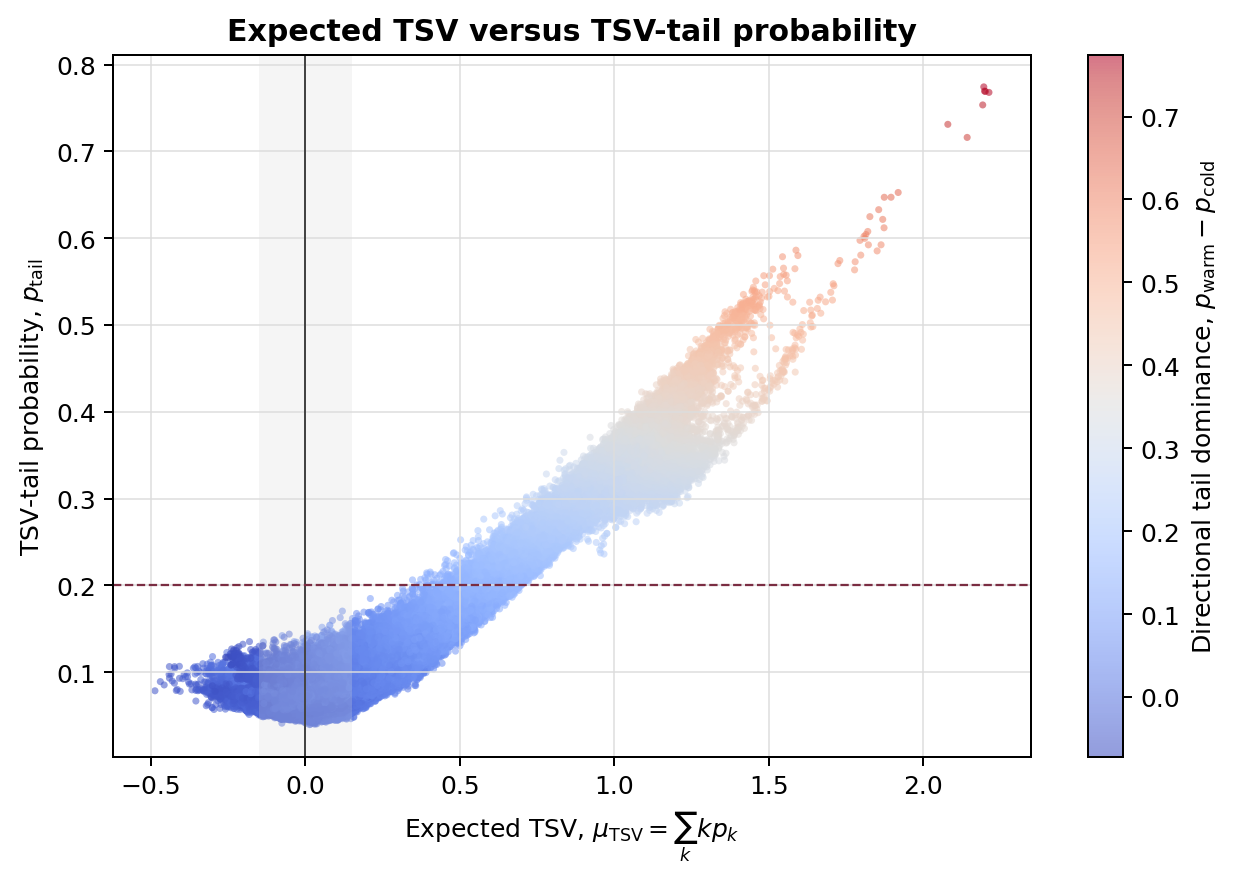
\includegraphics[width=0.86\linewidth]{figs/mean_vs_tail_scatter_sample.png}
    \caption{Expected TSV versus TSV-tail probability for a sampled subset of the 144-case diagnostic panel. Expected TSV denotes the probability-weighted mean $\mu_{\mathrm{TSV}}=\sum_k k p_k$, not the most likely TSV class. The horizontal line marks the illustrative reporting screen $p_{\mathrm{tail}}=0.20$. Expected TSV is informative, but $p_{\mathrm{tail}}$ directly reports the modeled probability mass in the selected TSV categories.}
    \label{fig:mean_tail_scatter}
\end{figure}

Figure~\ref{fig:mean_tail_scatter} shows the internal relationship between the TSV probability distribution and two summaries derived from it. Expected TSV remained strongly associated with TSV-tail probability, so the scalar mean is not meaningless. The diagnostic does not show near-neutral high-tail states under the strict condition $|\mu_{\mathrm{TSV}}|<0.15$; that share was 0.0\%. The stronger finding is different: similar positive mean states can still carry different tail probabilities. Within 0.05-wide expected-TSV bins, the 5th--95th percentile spread in $p_{\mathrm{tail}}$ reached 0.145 in the populated $\mu_{\mathrm{TSV}}=1.35$--1.40 bin ($n=1{,}204$). A scalar mean gives the warm-side tendency, but the probability distribution shows how much mass is assigned to the warm/hot outer categories.

The same figure also shows that TSV-tail probability in this fixed-reference panel is warm-dominant. Mean warm-tail probability was 0.088, compared with 0.027 for the cold tail. Warm-tail probability exceeded cold-tail probability in 78.3\% of occupied records and in all records crossing $p_{\mathrm{tail}}\ge0.20$. Records with $\mu_{\mathrm{TSV}}\le0$ never crossed the high-tail screen, while all records with $\mu_{\mathrm{TSV}}>1$ did. Thus, above about $+1$ expected TSV, the scalar mean already identifies a warm-tail state; the probability distribution is still needed to quantify the associated outer-category mass.

\subsection{PMV as a scalar benchmark}

The PMV comparison gives a second scalar benchmark. Across the same occupied records, $|\mathrm{PMV}|$ was correlated with $p_{\mathrm{tail}}$ (Pearson $r=0.859$, Spearman $\rho=0.752$), while $|\mu_{\mathrm{TSV}}|$ was more tightly correlated with $p_{\mathrm{tail}}$ (Pearson $r=0.975$, Spearman $\rho=0.895$). A best offline $|\mu_{\mathrm{TSV}}|$ threshold of 0.608 disagreed with the high-tail flag in 1.07\% of occupied records. A best offline $|\mathrm{PMV}|$ threshold of 0.913 disagreed in 3.27\% of occupied records.

\begin{figure}[H]
    \centering
    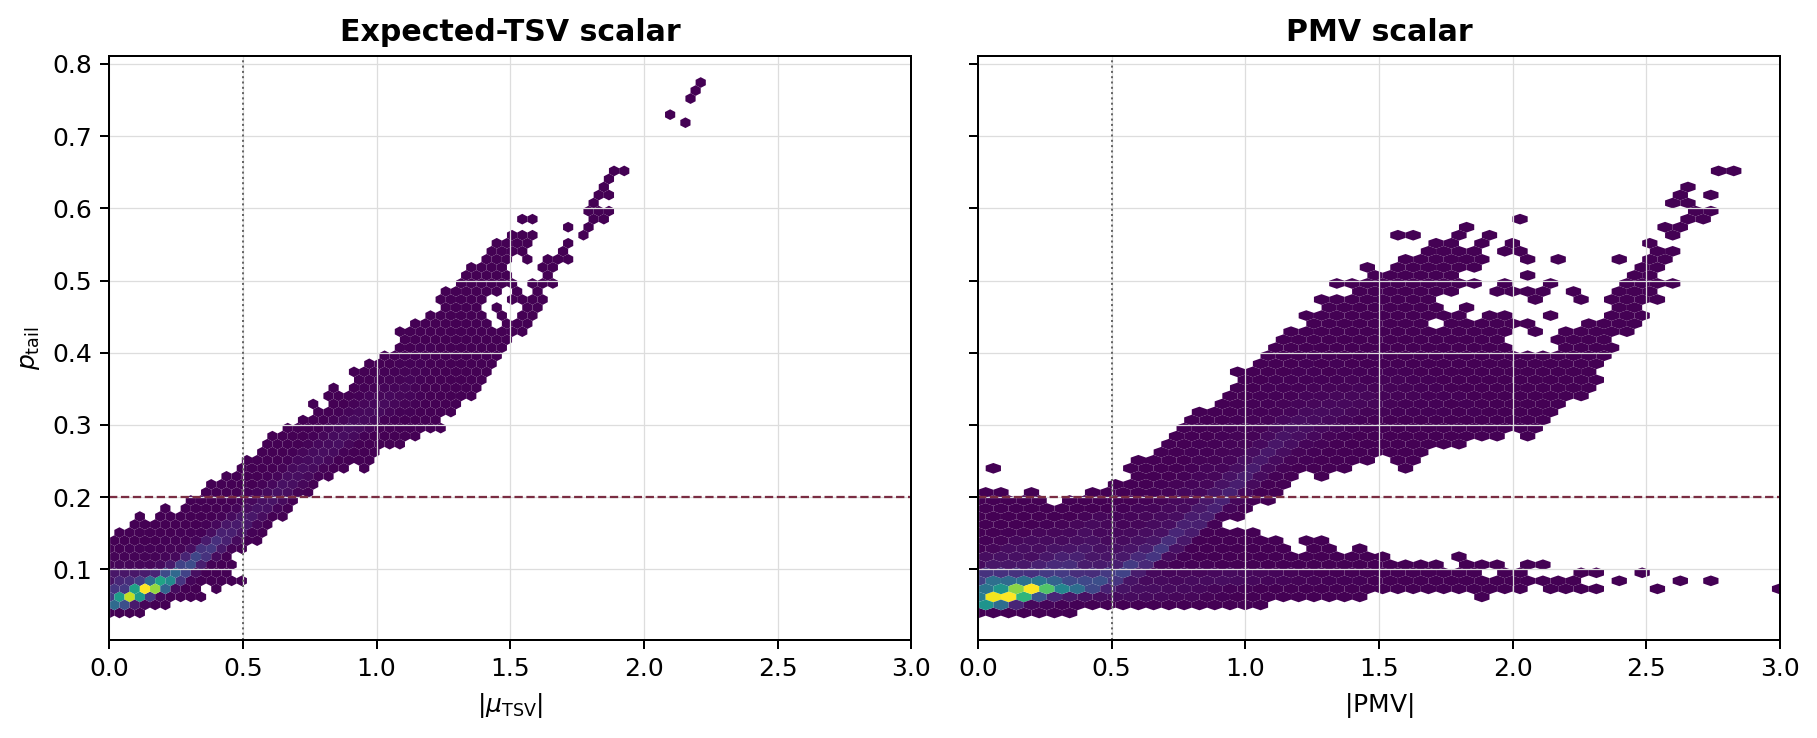
\includegraphics[width=\linewidth]{figs/scalar_tail_comparison_hexbin.png}
    \caption{Scalar comparison against the primary TSV probability output. Left: $|\mu_{\mathrm{TSV}}|$ versus $p_{\mathrm{tail}}$. Right: $|\mathrm{PMV}|$ versus the same $p_{\mathrm{tail}}$ distribution. Both panels use the same 0--3 scalar range. The vertical line marks the conventional 0.5 scalar band, and the horizontal line marks the diagnostic high-tail screen $p_{\mathrm{tail}}=0.20$.}
    \label{fig:pmv_scalar_comparison}
\end{figure}

\begin{table}[htbp]
\centering
\caption{Scalar threshold comparison against the $p_{\mathrm{tail}}\ge0.20$ high-tail flag. Best thresholds are optimized offline over the full diagnostic panel. Missed high-tail and false-positive rates are reported as percentages of all occupied records.}
\label{tab:pmv_scalar_comparison}
\scriptsize
\resizebox{\textwidth}{!}{%
\begin{tabular}{lrrrr}
\toprule
\textbf{Scalar rule} & \textbf{Threshold} & \textbf{Disagreement (\%)} & \textbf{Missed high-tail (\% records)} & \textbf{False positive (\% records)} \\
\midrule
$|\mu_{\mathrm{TSV}}|$ best threshold & 0.608 & 1.07 & 0.61 & 0.46 \\
$|\mathrm{PMV}|$ best threshold & 0.913 & 3.27 & 1.50 & 1.76 \\
$|\mathrm{PMV}|$ standard band & 0.500 & 18.93 & 0.003 & 18.92 \\
\bottomrule
\end{tabular}
}
\end{table}

Read together, Figures~\ref{fig:mean_tail_scatter} and~\ref{fig:pmv_scalar_comparison} separate two issues. Figure~\ref{fig:mean_tail_scatter} shows how the learned TSV expectation relates to its own tail probability. Figure~\ref{fig:pmv_scalar_comparison} asks how that relationship differs from PMV, Fanger's continuous comfort index built from thermal-balance terms and empirical chamber-vote evidence. The standard $|\mathrm{PMV}|=0.5$ band behaved conservatively in this panel. It almost never missed high-tail states, but it flagged many states that did not cross $p_{\mathrm{tail}}\ge0.20$. The learned expected-TSV scalar occupies a narrower range and follows the calibrated tail probability closely because both are summaries of the same seven-class probability vector. This is a tighter empirical association, not a claim of linearity: $|\mu_{\mathrm{TSV}}|$ reports the location of the predicted distribution, while $p_{\mathrm{tail}}$ reports its outer-category mass. Its maximum absolute value was 2.24 in this panel, and only 3.5\% of occupied records exceeded $|\mu_{\mathrm{TSV}}|=1$. PMV spans a wider scalar range, reaching 3.31 in absolute value, and includes a lower-$p_{\mathrm{tail}}$ branch at higher $|\mathrm{PMV}|$ values. This broad branch around $p_{\mathrm{tail}}\approx0.1$ is the visual source of the conservative PMV result: PMV can assign a large scalar departure to states that the calibrated TSV distribution still places mostly in neutral or mild categories. Among records with $|\mathrm{PMV}|\ge0.5$, 59.0\% remained below $p_{\mathrm{tail}}=0.20$; even among records with $|\mathrm{PMV}|\ge1$, 9.3\% remained below that tail-probability screen. The mid-tail band shows the same compression: for records with $0.3\le p_{\mathrm{tail}}<0.4$, the 5th--95th percentile range was 0.88--1.20 for $|\mu_{\mathrm{TSV}}|$ but 1.05--1.86 for $|\mathrm{PMV}|$. The point is not that PMV is useless or blind to thermal stress; rather, PMV and $p_{\mathrm{tail}}$ answer different diagnostic questions. PMV gives a conventional continuous mean-vote index for the thermal state. $p_{\mathrm{tail}}$ reports the predicted probability mass in the selected TSV categories.

The no-PMV robustness check gave the same qualitative result, but it should be read as a model-output comparison rather than as two versions of PMV. Figure~\ref{fig:pmv_feature_robustness} keeps the x-axis fixed as the same synchronized $|\mathrm{PMV}|$ scalar and changes the y-axis from the primary $p_{\mathrm{tail}}$ output to the $p_{\mathrm{tail}}$ output from a separately trained no-PMV TSV predictor. Removing PMV from the ordinal predictor changed the mean-zone high-tail exceedance at $p_{\mathrm{tail}}\ge0.20$ from 13.15\% to 13.85\%, and changed any-zone exceedance from 36.64\% to 37.52\%. The PMV-inclusive output is modestly tighter against the PMV scalar, with Pearson $r=0.859$ and Spearman $\rho=0.752$, compared with $r=0.857$ and $\rho=0.738$ for the no-PMV output. This supports a limited interpretation: calculable PMV is a useful predictor feature for reported TSV probabilities, but the main scalar-reference and aggregation results are not created solely by including PMV in the model. Under the no-PMV predictor, $|\mu_{\mathrm{TSV}}|$ still had Pearson $r=0.976$ with its own $p_{\mathrm{tail}}$ output. We therefore treat the PMV comparison as a descriptive scalar-reference audit, not as the main evidence for the probability diagnostic.

The saved nominal seven-class predictor provides a separate model-form check on the ordinal representation. At $p_{\mathrm{tail}}\ge0.20$, the nominal model's mean-zone, area-weighted mean-probability, p90-zone, and any-zone screened shares were 14.34\%, 12.74\%, 27.86\%, and 35.16\%, respectively, compared with 13.15\%, 12.13\%, 27.83\%, and 36.64\% for the ordinal model. The largest absolute rate difference was 1.48 percentage points, and both models preserved the ordering between mean, p90, and any-zone screens across the prespecified threshold range. The spatial conclusion is therefore a property of retaining categorical probabilities in this application, not an observed advantage that appears only under the cumulative ordinal algorithm.

\begin{figure}[htbp]
    \centering
    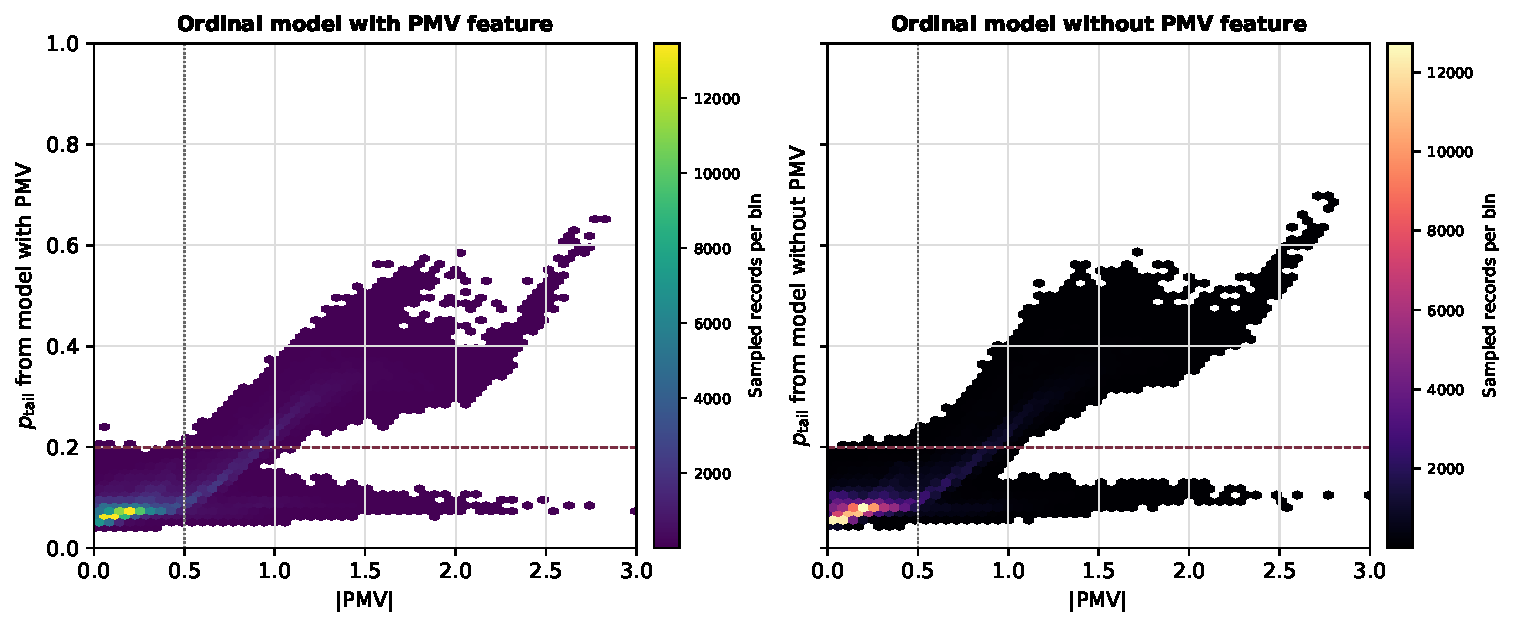
\includegraphics[width=\linewidth]{figs/pmv_feature_robustness_hexbin.pdf}
    \caption{PMV-scalar robustness check using two TSV probability outputs. Both panels use the same x-axis scalar, $|\mathrm{PMV}|$, from the simulated thermal state. The left panel plots PMV against $p_{\mathrm{tail}}$ from the primary TSV predictor, which includes PMV as an engineered covariate. The right panel plots the same PMV values against $p_{\mathrm{tail}}$ from a separately trained no-PMV TSV predictor. The different palettes indicate that the two panels contain different probability-model outputs, not different PMV calculations.}
    \label{fig:pmv_feature_robustness}
\end{figure}

For the probability metrics below, the Brier score is mean squared error of the binary tail probability; fixed-bin expected calibration error (ECE) is the bin-count-weighted absolute predicted--observed gap; area under the receiver operating characteristic curve (AUROC) and average precision summarize ranking discrimination; and F1 is the harmonic mean of precision and recall at the stated $p_{\mathrm{tail}}\ge0.20$ screen.

The pooled held-out TSV validation check gives the same practical reading (Tables~\ref{tab:tail_probability_comparison} and~\ref{tab:tsv_predictor_validation}). The primary and no-PMV predictors had nearly identical point performance: exact-class accuracy was 47.3\% and 46.9\%, within-one-class accuracy was 84.1\% and 83.8\%, and ordinal class MAE was 0.73 for both. The rounded-PMV class baseline was weaker on exact and ordinal metrics, with 33.2\% exact accuracy and 0.97 class MAE. Class-specific recall was modest in the tail classes for all methods, consistent with the neutral-heavy and noisy structure of field TSV data. Supplementary calibration checks show that aggregate predicted $p_{\mathrm{tail}}$ aligned closely with observed tail frequency on the held-out split: the primary model's mean predicted $p_{\mathrm{tail}}$ was 0.207 versus an observed tail frequency of 0.206, with fixed-bin tail ECE of 0.011. We also tested a PMV-only calibrated tail baseline, fitted as $|\mathrm{PMV}|\rightarrow\Pr(\mathrm{TSV}\le-2\ \mathrm{or}\ \mathrm{TSV}\ge+2)$ on the same non-test data. Table~\ref{tab:tail_probability_comparison} shows that this baseline matched overall tail prevalence but discriminated tail records less well than the TSV probability models. AUROC was 0.571 versus 0.747, average precision was 0.260 versus 0.483--0.487, Brier score was 0.161 versus 0.137--0.138, and F1 at the $p_{\mathrm{tail}}\ge0.20$ screen was 32.6\% versus 46.4--47.1\%. Contributor-clustered paired intervals preserved the primary model's advantage over the PMV-only baseline in Brier score, AUROC, and average precision, whereas every primary-versus-no-PMV interval included zero. A stricter contributor-grouped robustness check gave 42.1\% exact accuracy, 79.8\% within-one-class accuracy, tail AUROC of 0.577, and F1 of 32.5\%. This weaker transfer limits any absolute reading of simulated TSV-tail percentages under domain shift. The supported claim is therefore limited: primary and no-PMV held-out performance is similar, PMV alone contains useful but less discriminative tail information, and the diagnostic should not be treated as a PMV-only artifact.

An overlap-excluded reciprocal source-label holdout provided a separate domain-shift check. Six city--year strata with likely cross-source study overlap were removed from both corpora before refitting. Tail AUROC was 0.592 for ASHRAE-to-China and 0.553 in the reverse direction; tail ECE was 0.096 and 0.124, while mean predicted versus observed tail prevalence shifted from 0.225 versus 0.165 to 0.121 versus 0.223. Class-distance metrics did not consistently improve on an always-neutral target baseline. Transport therefore degraded materially across the two source labels. This check evaluates the fitting pipeline under source shift; the final pooled predictor has not been evaluated on a wholly unused third corpus.

\begin{table}[htbp]
\centering
\caption{Held-out tail-probability comparison for the TSV probability models and the PMV-only calibrated scalar baseline. F1 is computed by screening each predicted tail probability at $p_{\mathrm{tail}}\ge0.20$.}
\label{tab:tail_probability_comparison}
\scriptsize
\setlength{\tabcolsep}{4.2pt}
\begin{tabular}{lrrrrrr}
\toprule
\textbf{Predictor} & \textbf{Mean predicted} & \textbf{Observed} & \textbf{Brier} & \textbf{ECE} & \textbf{F1 (\%)} & \textbf{AUROC} \\
\midrule
Primary TSV model & 0.207 & 0.206 & 0.137 & 0.011 & 47.1 & 0.747 \\
No-PMV TSV model & 0.207 & 0.206 & 0.138 & 0.006 & 46.4 & 0.747 \\
PMV-only calibrated tail baseline & 0.206 & 0.206 & 0.161 & 0.003 & 32.6 & 0.571 \\
\bottomrule
\end{tabular}
\end{table}

\begin{table}[htbp]
\centering
\caption{Held-out TSV class validation for the primary predictor, the no-PMV robustness predictor, and a rounded-PMV class baseline. The PMV baseline rounds PMV to the nearest TSV class and clips to $[-3,+3]$; it is a deterministic scalar-label baseline, not a probability model. Argmax-tail F1 converts each probability vector to its most probable class before grouping classes by tail status; it is distinct from F1 at the probability screen reported in Table~\ref{tab:tail_probability_comparison}. Class recall columns report the share of records in each observed TSV class assigned to that same class.}
\label{tab:tsv_predictor_validation}
\scriptsize
\resizebox{\textwidth}{!}{%
\begin{tabular}{lrrrrrrrrrrrr}
\toprule
\textbf{Predictor} & \textbf{Exact (\%)} & \textbf{Within $\pm1$ (\%)} & \textbf{Class MAE} & \textbf{Argmax-tail F1 (\%)} & \textbf{Log loss} & \textbf{TSV -3} & \textbf{TSV -2} & \textbf{TSV -1} & \textbf{TSV 0} & \textbf{TSV +1} & \textbf{TSV +2} & \textbf{TSV +3} \\
\midrule
Primary TSV model & 47.3 & 84.1 & 0.73 & 34.0 & 1.454 & 25.5 & 6.9 & 12.4 & 88.0 & 16.2 & 15.7 & 23.9 \\
No-PMV TSV model & 46.9 & 83.8 & 0.73 & 33.5 & 1.476 & 23.7 & 6.5 & 13.0 & 87.4 & 15.4 & 15.8 & 23.2 \\
Rounded PMV class & 33.2 & 76.5 & 0.97 & 26.6 & -- & 13.8 & 10.4 & 27.6 & 47.8 & 26.3 & 14.5 & 10.5 \\
\bottomrule
\end{tabular}
}
\end{table}

\subsection{Zone aggregation hides localized tail exceedance}

Mean-zone and area-weighted summaries were similar in magnitude, but they also hid localized high-tail states. Across the full panel, the mean-zone probability screen identified 13.15\% high-tail exceedance. The area-weighted mean-probability screen, which thresholds after spatial probability averaging, identified 12.13\%; the distinct area-weighted zone-time screened share, which area-weights zone-level binary screens before time averaging, was 12.87\%. In 23.50\% of occupied records, however, the mean-zone value was below $p_{\mathrm{tail}}=0.20$ while at least one localized zone exceeded it. These are modeled occupied-timestep zone-state exceedances, not measured occupant exposures. Any-zone exceedance should therefore be read as a spatial screening statistic rather than as an occupant-prevalence estimate; it is intentionally sensitive to localized perimeter-zone states and is interpreted alongside p90-zone and the two area-weighted summaries. For context, any-zone aggregation identified 36.64\% high-tail exceedance, and p90-zone aggregation identified 27.83\%. Under the prespecified three-level probability categorization, a maximum-zone summary assigned a higher category than the mean in 32.05\% of occupied records; a p90-zone summary did so in 21.08\%.

\begin{figure}[H]
    \centering
    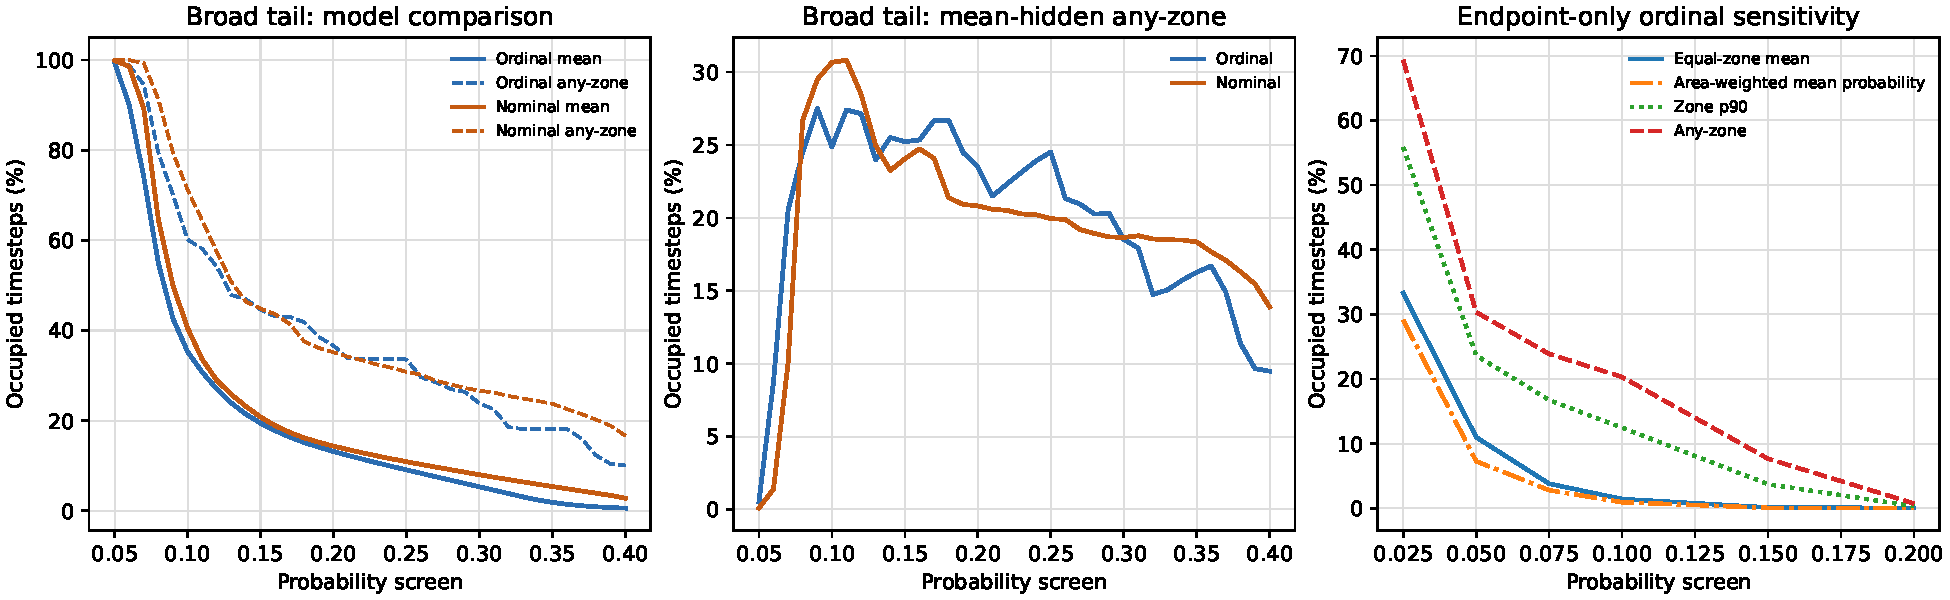
\includegraphics[width=0.66\linewidth]{figs/p_tail_threshold_sensitivity.pdf}
    \caption{Probability-screen and tail-definition sensitivity across the full 144-role fixed-reference panel. Left: mean-zone and any-zone screened shares for the primary ordinal and nominal seven-class predictors. Center: the corresponding mean-hidden any-zone share. Right: mean-zone, area-weighted mean-probability, p90-zone, and any-zone screened shares for the endpoint-only probability $p_{\mathrm{outermost}}=\Pr(\mathrm{TSV}\in\{-3,+3\})$. Absolute shares are model-, threshold-, and event-definition-conditional, while the mean-to-any-zone ordering persists across the tested specifications.}
    \label{fig:tail_threshold_sensitivity}
\end{figure}

Figure~\ref{fig:tail_threshold_sensitivity} tests whether this hidden-zone effect depends on the selected reporting screen, predictor form, or tail definition. For the primary tail, absolute exceedance falls as the screen becomes stricter, but any-zone exceedance remains well above mean-zone exceedance. At $\tau=0.10$, mean-zone exceedance was 35.30\% and any-zone exceedance was 60.18\%; at $\tau=0.30$, they were 5.30\% and 23.83\%, respectively. Hidden any-zone exceedance remained at least 18.5\% from $\tau=0.10$ to 0.30. The nominal predictor preserved the same spatial ordering, although model differences in absolute rates were threshold-dependent and reached 11.05 percentage points for the any-zone statistic at $\tau=0.10$. The no-PMV predictor also showed the same pattern: at $\tau=0.20$, mean-zone exceedance was 13.85\%, any-zone exceedance was 37.52\%, and hidden any-zone exceedance was 23.67\%.

The endpoint-only event provides a stricter category-boundary check. At an endpoint-probability screen of 0.05, mean-zone exceedance was 10.99\%, any-zone exceedance was 30.34\%, and the mean-hidden any-zone share was 19.35\%. Across the prespecified endpoint screens from 0.025 to 0.20, the paired any-zone-minus-mean-zone gap remained positive; its conditional bootstrap range narrowed from 36.03 [34.58, 37.48] percentage points at 0.025 to 0.70 [0.41, 1.04] at 0.20. Because the held-out corpus contains only 1{,}350 endpoint observations among 22{,}223 test records, this result is a support-limited bounding sensitivity, not a replacement outcome.

The area-weighted zone-time diagnostic gives a useful check on this result. Its close agreement with the mean-zone value does not remove the localized high-tail signal. It shows that much of the hidden any-zone exceedance comes from smaller perimeter zones rather than from the largest core zones.

\begin{table}[htbp]
\centering
\caption{Zone aggregation summary by city. Mean, any-zone, and p90-zone columns report modeled high-tail exceedance at $p_{\mathrm{tail}}\ge0.20$. Any-zone exceedance is the share of occupied timesteps for which the maximum zone value satisfies $\max_z p_{\mathrm{tail},z}\ge0.20$. Hidden high-tail exceedance means the mean-zone value is below 0.20 while at least one zone is at or above 0.20.}
\label{tab:zone_aggregation_summary}
\scriptsize
\resizebox{\textwidth}{!}{%
\begin{tabular}{lrrrrr}
\toprule
\textbf{City} & \textbf{Mean-zone (\%)} & \textbf{Area-weighted zone-time (\%)} & \textbf{Any-zone (\%)} & \textbf{p90-zone (\%)} & \textbf{Hidden any-zone (\%)} \\
\midrule
Ahmedabad & 16.65 & 17.21 & 53.88 & 41.63 & 37.22 \\
Beijing & 5.37 & 5.75 & 15.44 & 9.86 & 10.07 \\
Guangzhou & 12.22 & 11.63 & 31.70 & 22.90 & 19.47 \\
Houston & 12.09 & 10.81 & 27.82 & 22.00 & 15.73 \\
Kolkata & 19.53 & 20.36 & 46.80 & 35.92 & 27.26 \\
Phoenix & 13.02 & 11.48 & 44.23 & 34.67 & 31.22 \\
\bottomrule
\end{tabular}
}
\end{table}

The zones with the largest high-tail screened shares were perimeter zones, especially P1, the south perimeter orientation in this DOE Medium Office geometry. The largest high-tail exceedance rates were 30.24\% for \texttt{perimeter\_bot\_zn\_1}, 27.62\% for \texttt{perimeter\_mid\_zn\_1}, and 23.27\% for \texttt{perimeter\_top\_zn\_1}. Each of these zones accounts for about 4.16\% of conditioned floor area, while each core zone accounts for about 19.74\%. Thus, the largest modeled local tail exceedance occurs in relatively small perimeter zones, while the building-level area-weighted signal is shaped strongly by the larger core zones.

Figure~\ref{fig:zone_size_mosaic} shows that this local pattern changes by city and time slice. Beijing remains comparatively low: the largest pooled zone-specific screened share rises from 7.1\% in the reference slice to 14.9\% in the late-2080s slice. Guangzhou shows a clearer future-weather transition, with its largest zone-specific share increasing from 20.2\% in the reference slice to 28.9\% in the mid-2050s and 41.7\% in the late-2080s. Kolkata reaches higher exceedance earlier: its corresponding value is 31.5\% in the reference slice, 48.2\% in the mid-2050s, and 55.4\% in the late-2080s. Ahmedabad has a different structure: south-perimeter P1 already has a high screened share, but non-P1 perimeter and core zones remain much lower until the late-2080s. This is why Ahmedabad can appear high under an any-zone view while the broader zone field is less uniformly elevated than Kolkata.

\begin{figure}[p]
    \centering
    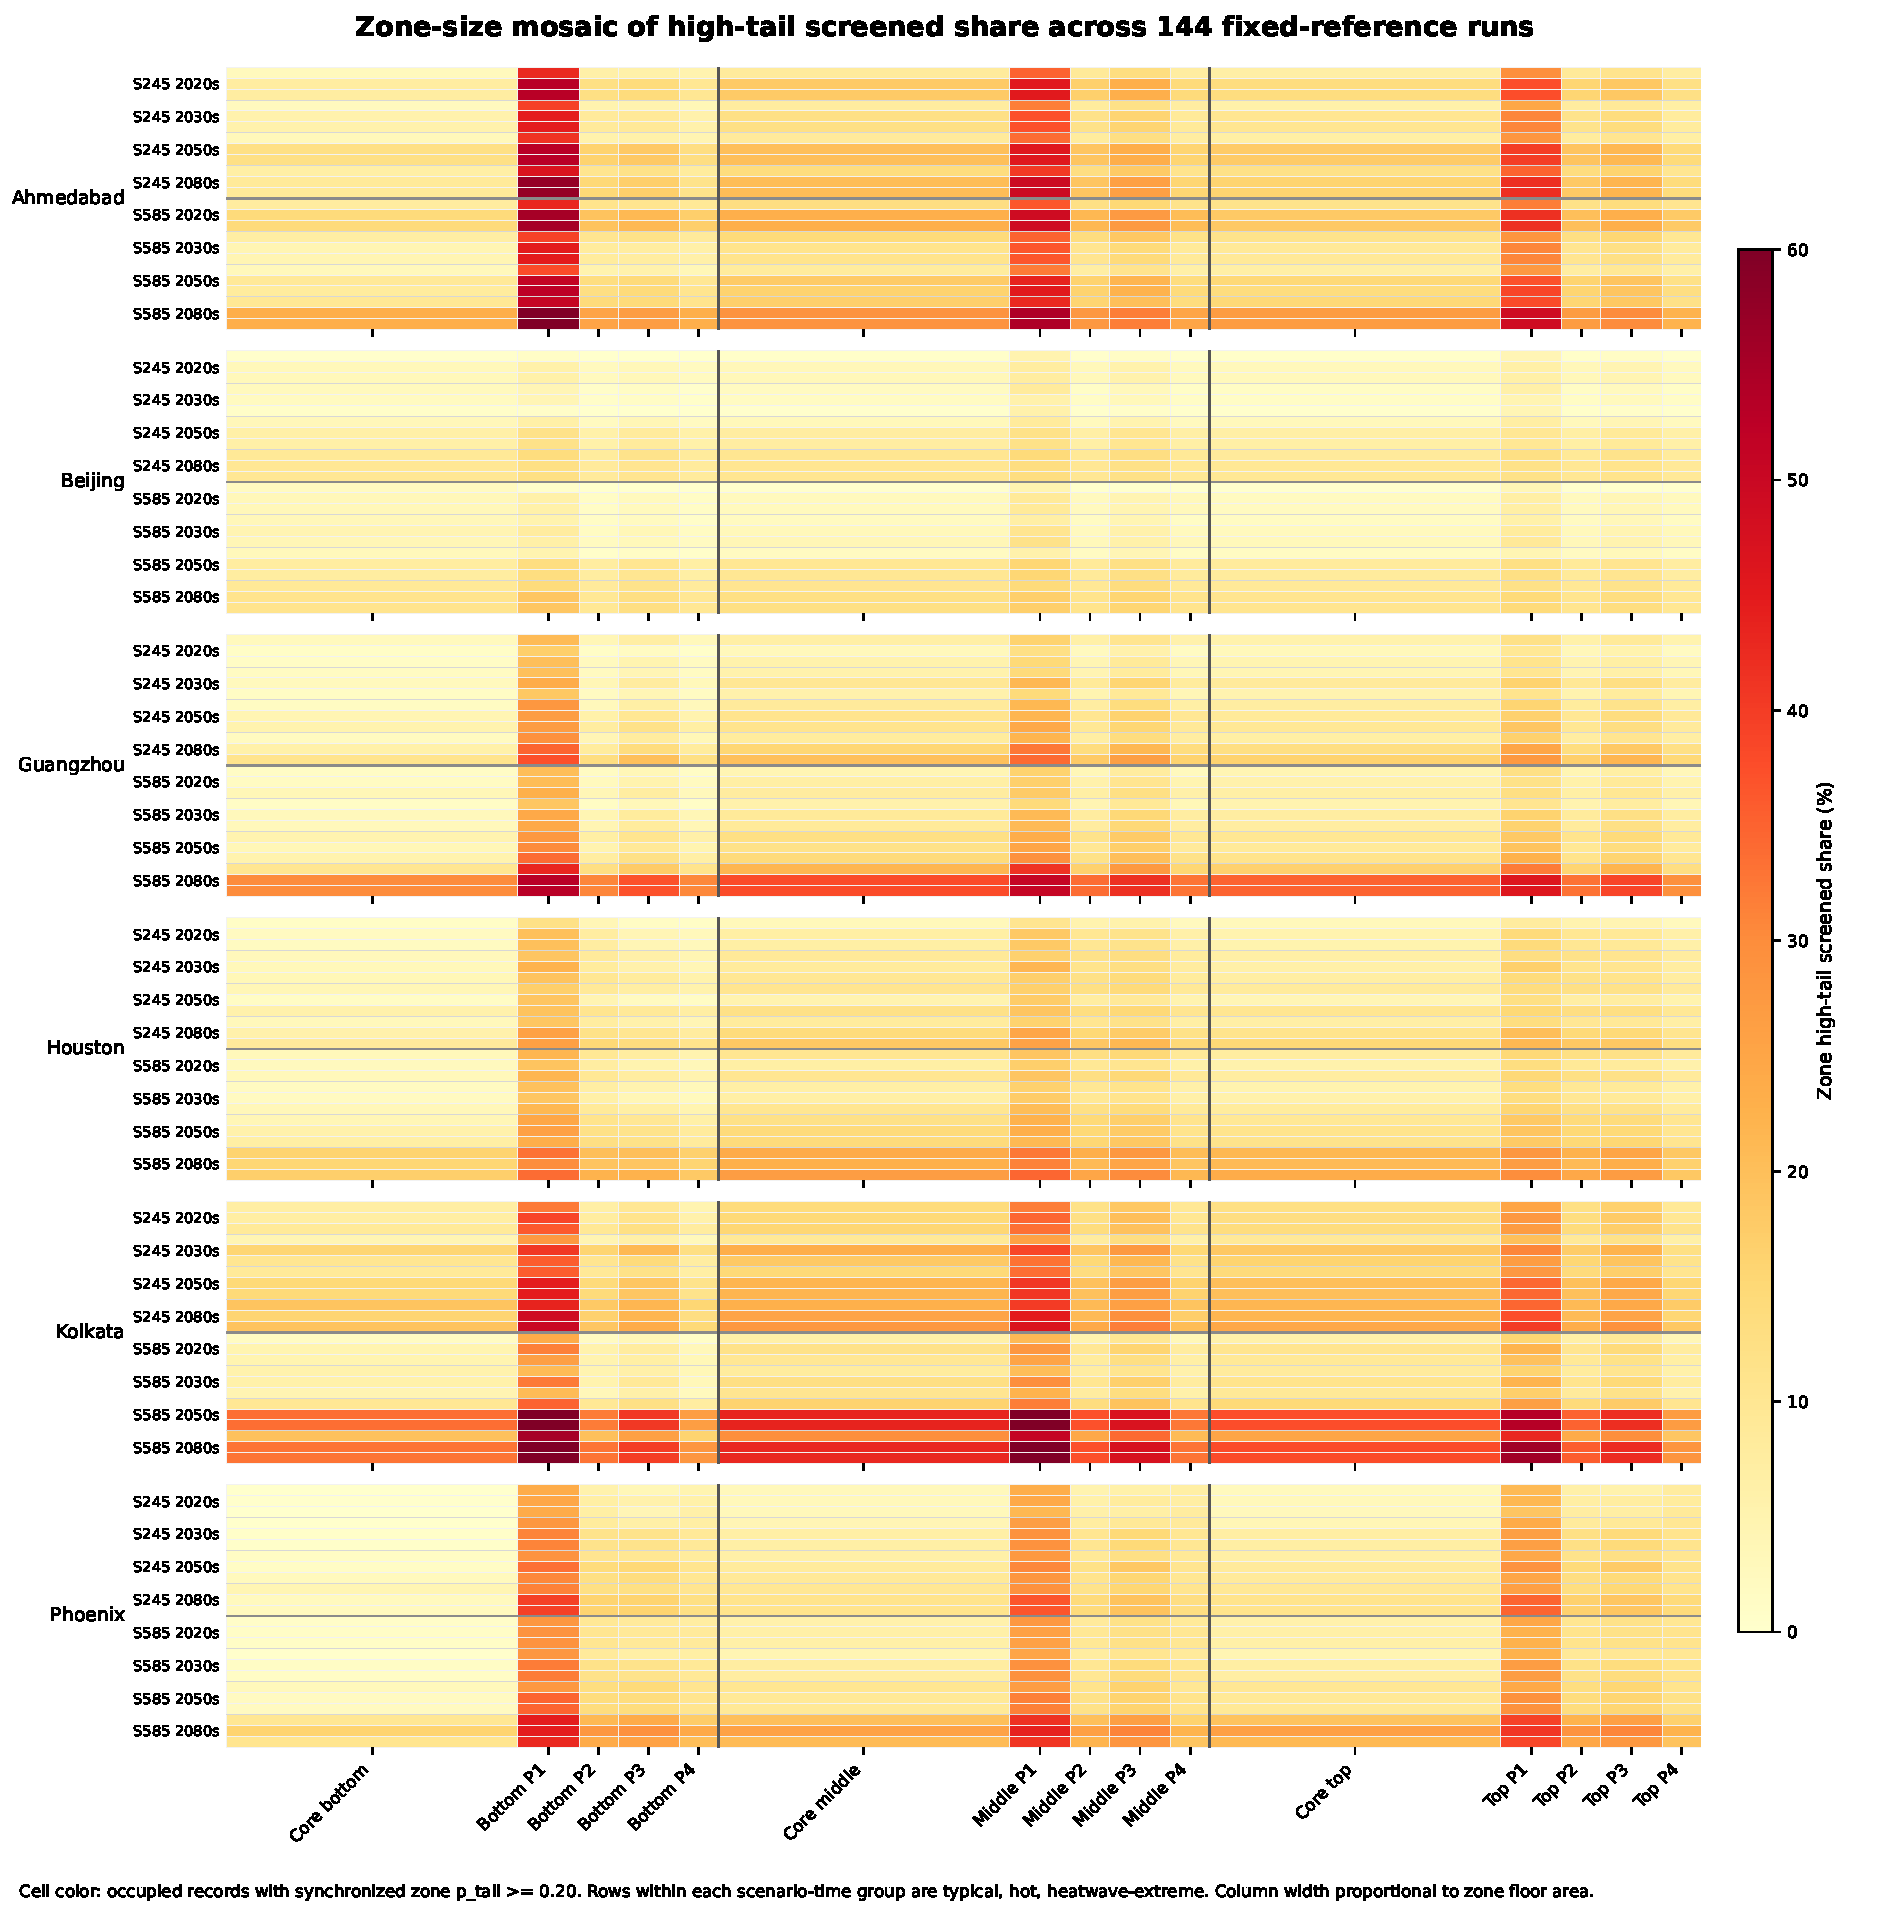
\includegraphics[width=\linewidth,height=0.86\textheight,keepaspectratio]{figs/zone_size_mosaic_heatmap_area.pdf}
    \caption{Zone-size mosaic of modeled high-tail exceedance across the 144-case fixed-reference panel. Cell color reports the share of occupied records in each case-zone pair with $p_{\mathrm{tail}}\ge0.20$. Column width is proportional to conditioned floor area, so the figure compares local tail exceedance with the physical size of the zone carrying that signal. Core bottom, core middle, and core top are the three core zones of the DOE Medium Office prototype; Bottom P1--P4, Middle P1--P4, and Top P1--P4 are the four perimeter zones on each floor level. P1--P4 denote perimeter orientations: P1 south, P2 east, P3 north, and P4 west. The conditioned top zones sit below the top-floor plenum and roof assembly, so ``top'' should not be read as a directly roof-exposed room condition. Rows within each scenario-time group are ordered as typical, hot, and heatwave-extreme weather files.}
    \label{fig:zone_size_mosaic}
\end{figure}

Figure~\ref{fig:zone_floor_position} was generated as a direct check on the floor/orientation reading from Fig.~\ref{fig:zone_size_mosaic}. It prevents over-reading the mosaic as a simple floor-height effect. Area-weighted high-tail exceedance was 10.79\% for the bottom floor, 14.79\% for the middle floor, and 13.03\% for the top floor. The middle floor had the highest area-weighted floor exceedance in 135 of 144 cases. Bottom-floor exceedance was highest only under an any-zone-within-floor summary, where the south perimeter zone P1 dominated. Bottom P1 had 30.24\% high-tail exceedance, compared with 27.62\% for middle P1 and 23.27\% for top P1. For the other perimeter orientations, bottom was not the highest. We therefore interpret the floor pattern as a prototype-specific interaction between perimeter orientation, floor construction, and zone conditioning, not as a general result that lower floors have higher screened shares than upper floors. High-tail states were warm-dominant in all zones under the $p_{\mathrm{tail}}\ge0.20$ screen.

\begin{figure}[htbp]
    \centering
    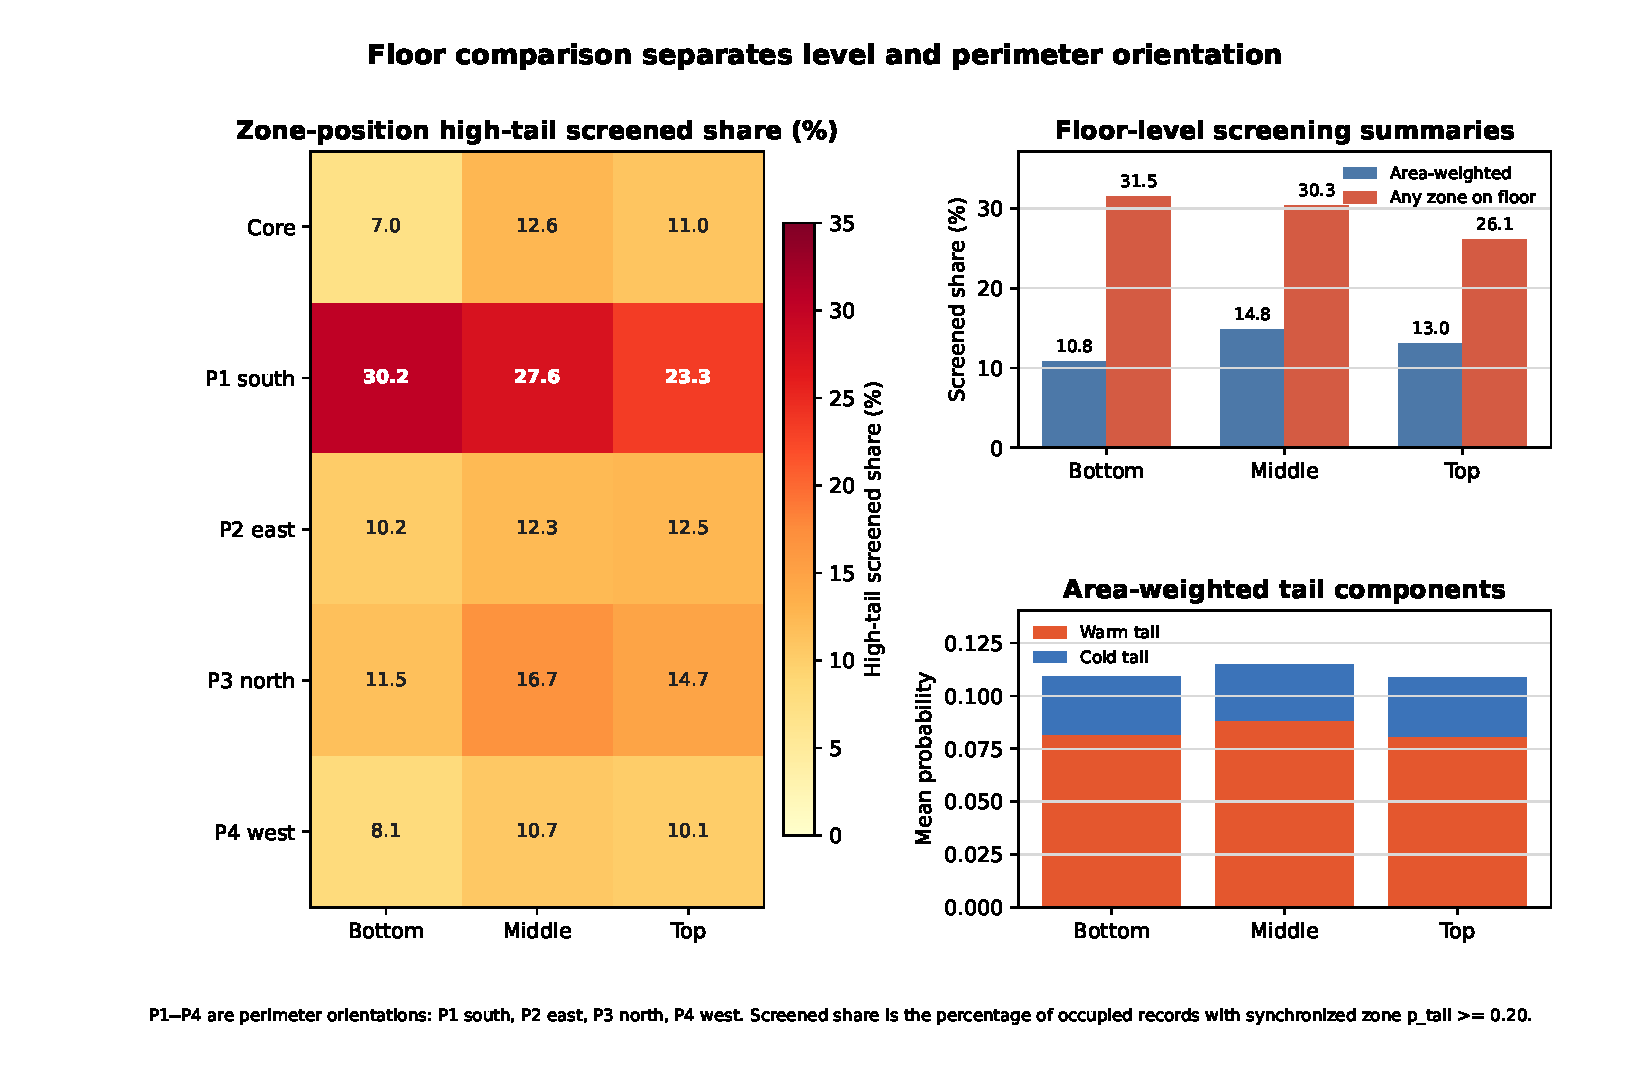
\includegraphics[width=\linewidth]{figs/zone_floor_position_comparison.pdf}
    \caption{Floor-position comparison for the 144-case fixed-reference panel. The heat map reports modeled high-tail exceedance by floor and zone position. P1--P4 are the perimeter orientations in the DOE Medium Office prototype: P1 south, P2 east, P3 north, and P4 west. Area-weighted floor exceedance summarizes zone-time records using conditioned floor area, while any-zone floor exceedance reports the share of occupied records in which at least one zone on that floor exceeds $p_{\mathrm{tail}}\ge0.20$. Tail-component bars show that floor differences are driven mainly by the warm tail.}
    \label{fig:zone_floor_position}
\end{figure}

\subsection{Weather-to-zone association audit}

The recorded states support a mechanism-consistent three-link interpretation, although not causal decomposition. Across the 144 role-labelled cases, the median within-case Spearman association between outdoor dry-bulb temperature and mean-zone operative temperature was 0.824 (interquartile range 0.753--0.897). The median association between operative temperature and $p_{\mathrm{tail}}$ was 0.855 (0.794--0.917), while the descriptive association between requested zone cooling rate and $p_{\mathrm{tail}}$ was 0.574 (0.411--0.629). The cooling association indicates coincident HVAC response; without unmet-load or component-capacity outputs it does not establish plant saturation.

Matched baseline-to-late comparisons make the pathway clearer. Annual mean outdoor temperature, occupied mean-zone operative temperature, mean $p_{\mathrm{tail}}$, and mean-zone screened share all increased in 36 of 36 city--scenario--selection-role comparisons. The median changes were $+2.13$\,\degree C outdoors, $+0.50$\,\degree C operative, $+0.0259$ in mean $p_{\mathrm{tail}}$, and $+10.13$ percentage points in screened share. After duplicate roles were collapsed, screened share increased from 0.19\% in the 20--25\,\degree C outdoor-temperature stratum to 52.69\% at outdoor temperatures of at least 35\,\degree C. Across the same 119 unique states, the three south-perimeter zones averaged 25.93\% high-tail exceedance, compared with 11.21\% for the other nine perimeter zones.

Whole-year correlations should not be read as temperature-response coefficients. Ten of 144 annual operative-temperature--total-tail correlations were negative, all in Beijing, because whole-year season mixing interacts with the predictor's running-mean outdoor context and other covariates. Under outdoor temperature at or above 25\,\degree C, however, the operative-temperature--warm-tail association was positive in every case, with median $\rho=0.977$. The combined evidence is therefore consistent with hotter selected weather shifting simulated operative conditions and warm-tail probability while the fixed HVAC system responds. It does not isolate facade solar gain, humidity, envelope heat flux, or equipment capacity as independent causes.

\subsection{Metabolic-input sensitivity}

The metabolic-input sensitivity shows that representative occupant assumptions can materially change the TSV-tail profile even when the simulated thermal environments are held fixed. Table~\ref{tab:metabolic_scenario_summary} is a panel-level summary across both SSP pathways, all six cities, four time slices, and three annual weather severities; it is not a pathway-specific estimate. Across 216{,}483{,}840 zone-profile probability evaluations, the mean spread in mean-zone $p_{\mathrm{tail}}$ across the six metabolic profiles was 0.074, with a 95th percentile spread of 0.209. For max-zone $p_{\mathrm{tail}}$, the mean spread was 0.137 and the 95th percentile spread was 0.327.

Changing the metabolic profile also changed threshold status. Mean-zone high-tail status flipped across metabolic profiles in 18.99\% of occupied records, and max-zone high-tail status flipped in 38.66\%. When the S-real profile remained below the high-tail cutoff, some other metabolic profile crossed it in 18.80\% of mean-zone records and 36.51\% of any-zone records. Because the fixed-reference panel is warm-tail dominated, lower metabolic-load profiles generally reduced the predicted high-tail screened share. In this diagnostic, a lower metabolic input means the same simulated thermal environment is interpreted by the reported-TSV model with less occupant metabolic heat.

\begin{table}[htbp]
\centering
\caption{Panel-level metabolic-spread results across the full 144-case fixed-reference panel: six cities, SSP2-4.5 and SSP5-8.5, four time slices, and three annual weather severities. Values are pooled across pathways and recomputed over fixed environmental traces; EnergyPlus was not rerun with altered occupant heat gains.}
\label{tab:metabolic_scenario_summary}
\footnotesize
\begin{tabular}{lrrrr}
\toprule
\textbf{Profile} & \textbf{W/person} & \textbf{met} & \textbf{Mean-zone high-tail (\%)} & \textbf{Any-zone high-tail (\%)} \\
\midrule
COMP-Lo & 90.0 & 0.900 & 3.32 & 13.82 \\
S-real & 93.2 & 0.932 & 3.10 & 14.89 \\
COMP-Med & 100.0 & 1.000 & 7.97 & 29.78 \\
EQ-Max & 108.0 & 1.080 & 21.20 & 45.37 \\
COMP-Hi & 110.0 & 1.100 & 13.66 & 38.44 \\
LEGACY & 120.0 & 1.200 & 17.32 & 47.87 \\
\bottomrule
\end{tabular}
\end{table}

The response is not strictly monotone across all adjacent profiles; in particular, the calibrated model gives a lower mean-zone high-tail screened share at 110 W/person than at 108 W/person. We therefore interpret this section as a sensitivity diagnostic across metabolic assumptions, not as a smooth physiological dose-response curve. The practical result is still clear: the single representative occupant assumption can hide a substantial range of predicted reported-TSV tail screening.

The zone-resolved profile summaries show where this sensitivity is concentrated. Across the 2{,}160 case-zone summaries for each profile, the mean case-zone high-tail screened share was 3.27\% for COMP-Lo, 3.26\% for S-real, 8.65\% for COMP-Med, 19.25\% for EQ-Max, 15.37\% for COMP-Hi, and 18.77\% for LEGACY. The spread in case-zone screened share across the six profiles averaged 16.85 percentage points, with a 95th percentile of 36.15 percentage points. The largest mean spreads occurred in the south perimeter zones: Bottom P1 (30.44 percentage points), Middle P1 (28.64 percentage points), and Top P1 (24.96 percentage points). This reinforces the diagnostic claim: metabolic assumptions and zone aggregation interact, so a single representative occupant can hide spatially localized profile sensitivity.

\begin{figure}[htbp]
    \centering
    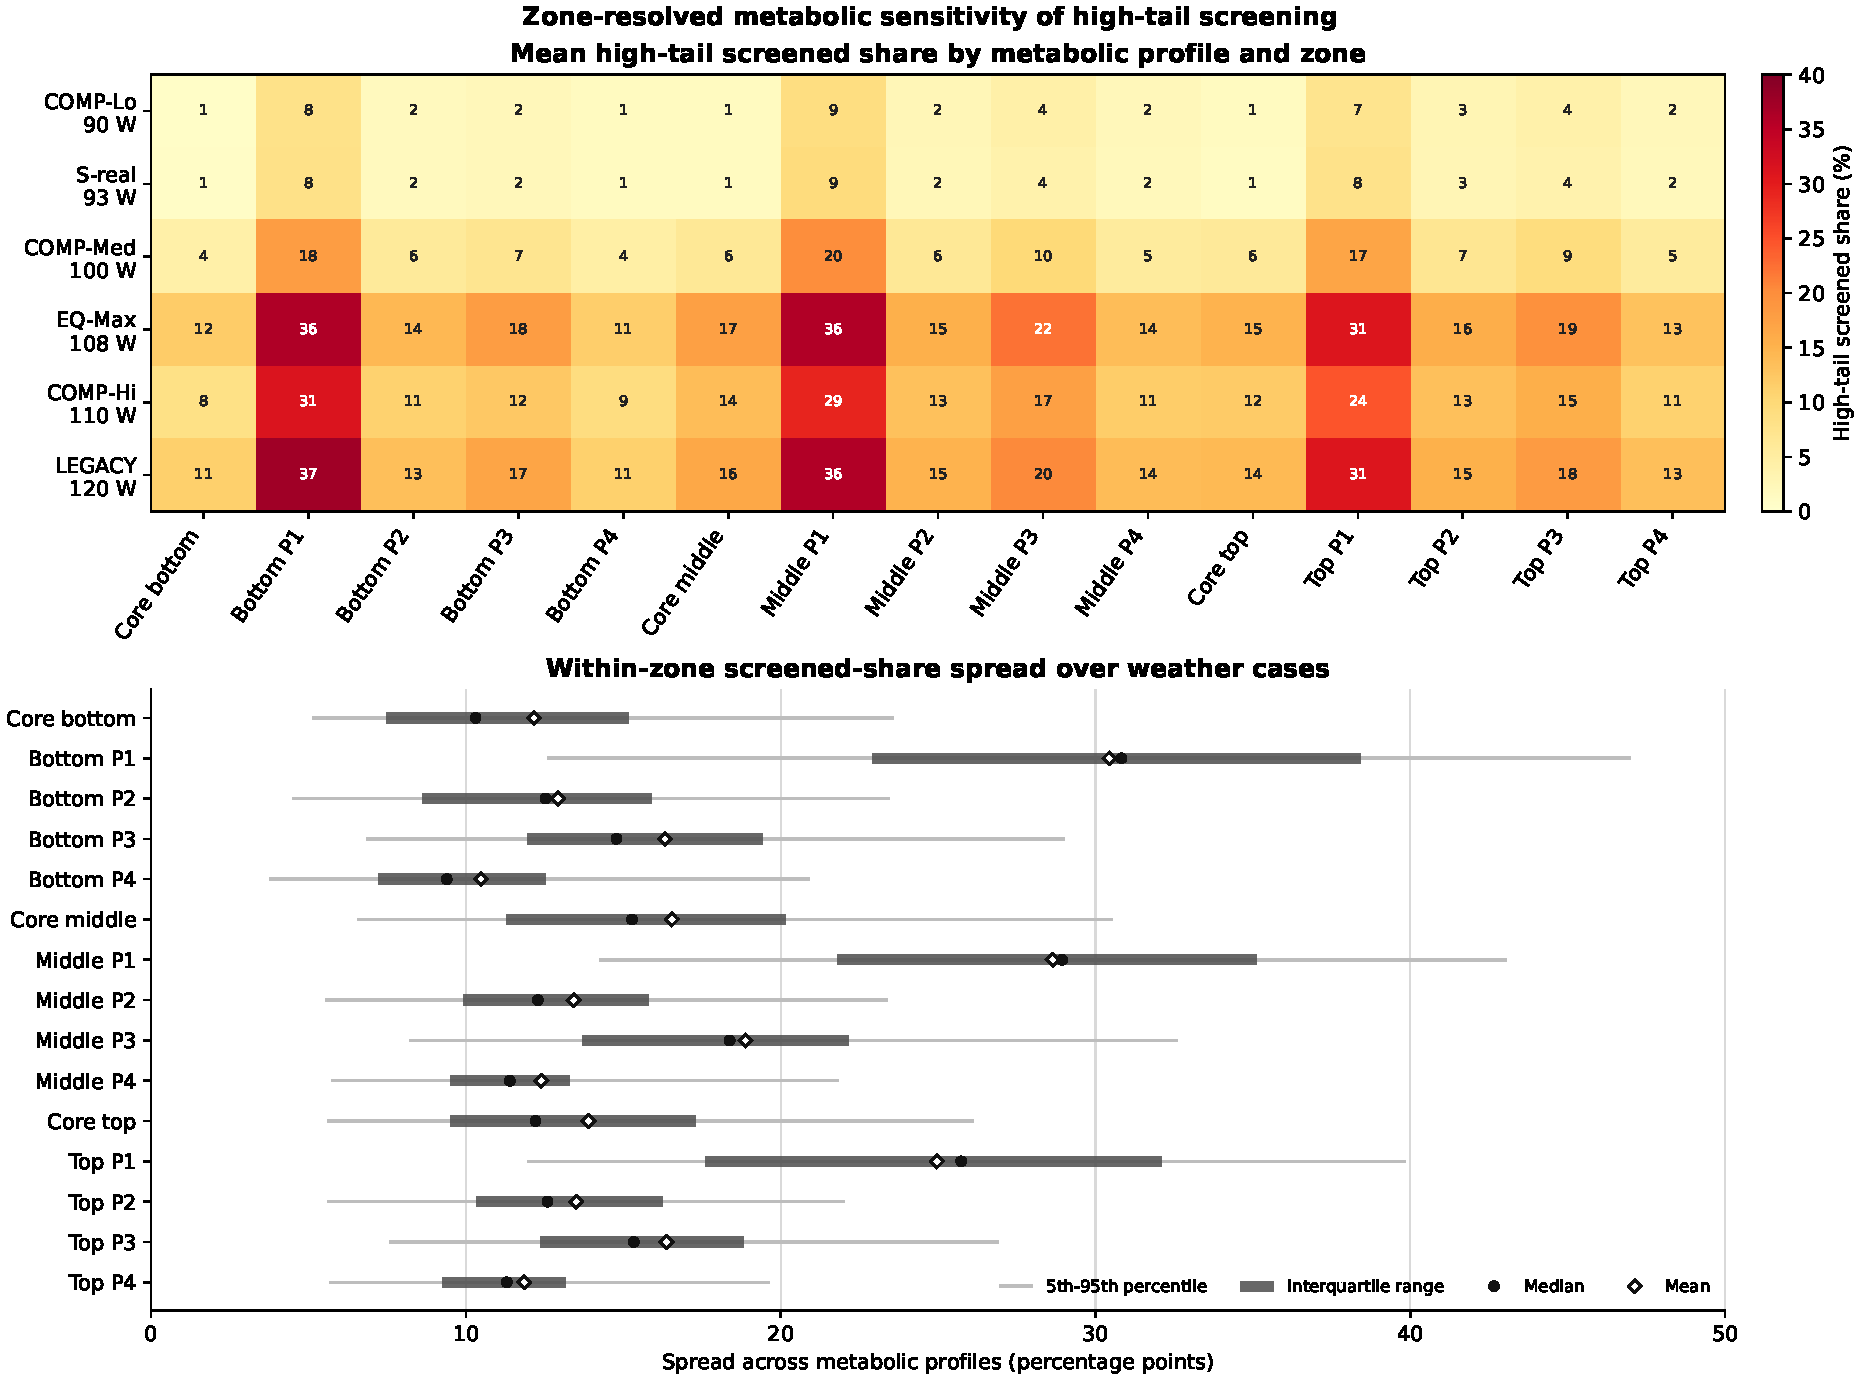
\includegraphics[width=\linewidth]{figs/zone_metabolic_profile_summary.pdf}
    \caption{Zone-resolved metabolic sensitivity of high-tail screening. Top: mean case-zone screened share by metabolic profile and zone. Bottom: within-zone spread across metabolic profiles summarized over the 144 weather cases. Points mark medians, diamonds mark means, thick intervals show the interquartile range, and thin intervals show the 5th--95th percentile range. Values are recomputed over fixed simulated environments, so the differences reflect representation sensitivity to metabolic inputs rather than altered internal heat gains or measured occupant exposure.}
    \label{fig:metabolic_profile_summary}
\end{figure}

\clearpage
\section{Discussion}\label{discuss}

\subsection{What the probability diagnostic adds}

The main contribution is not a new HVAC method. It is a diagnostic interface for reading a calibrated TSV probability distribution. Expected TSV, defined as the probability-weighted mean $\mu_{\mathrm{TSV}}=\sum_k k p_k$, remains useful: in the full panel it was strongly associated with $p_{\mathrm{tail}}$, and the diagnostic did not produce near-neutral high-tail states under $|\mu_{\mathrm{TSV}}|<0.15$. This is an important constraint on the interpretation. The probability representation does not overturn the scalar mean.

The added value is that the distribution makes tail probability explicit. A scalar mean reports central tendency; $p_{\mathrm{tail}}$ reports the probability mass in the selected cool/cold and warm/hot categories. Similar mean states can still have different tail probabilities, and the threshold status of $p_{\mathrm{tail}}$ is directly available only when the distribution is retained. In this fixed-reference future-weather panel, the visible tail was also strongly warm-skewed: cold-tail probability was small, and high-tail records were warm-dominant. That pattern is conditional on the selected cities, weather files, fixed thermostat schedule, and static comfort model, but it is exactly the kind of directional diagnostic that the probability object makes explicit.

The panel summary in Table~\ref{tab:panel_tail_summary} also matters because it separates broad stress-test gradients from local case differences. High-tail exceedance was similar in the reference and near-2030s slices, then increased in the mid-2050s and late-2080s; it was also higher under SSP5-8.5 than SSP2-4.5. The typical-year selector followed the same time-slice ordering, while the hot and heatwave-extreme annual files were close in aggregate exceedance. The city spread was larger than either scenario contrast or annual-severity contrast. This supports a cautious reading: the fixed archetype shows more high-tail states in the later selected weather, but the diagnostic should not be reduced to a single climate-scenario ranking. Local climate, selected annual file, and building-zone response still shape the observed tail profile.

The weather-to-zone audit supplies a physical pathway for that descriptive gradient. All 36 matched reference-to-late role comparisons moved toward warmer outdoor and simulated operative conditions and higher mean tail probability, and the direction also held in all 12 city--scenario cells after duplicate weather roles were collapsed. The cooling system responded concurrently, but the available traces do not establish equipment saturation. Likewise, the south-perimeter concentration is consistent with orientation, envelope, and zoning interaction in this prototype, but horizontal GHI cannot identify facade-incident solar causation. These safeguards are important because the fitted probability model also conditions on humidity and running-mean outdoor context: whole-year rank associations describe seasonal co-movement, not a causal temperature coefficient.

\subsection{Interpretation of the discomfort-relevant TSV tail}

The \(|\mathrm{TSV}|\ge2\) category boundary is not an assertion that every warm or cool vote is unacceptable. It is a convention-anchored screening construct. On the seven-point scale, \(+1\) is ``slightly warm'' and remains in the central band used here; \(+2\) is ``warm.'' The PMV--PPD lineage associates the \(\pm2\) and \(\pm3\) sensation categories with dissatisfaction, which makes the selected tail relevant to comfort screening \citep{Fanger1970PMV,ASHRAE2023}. That historical grouping anchors the boundary but does not turn a sensation vote into a directly observed satisfaction, preference, or acceptability response.

This distinction is especially important under adaptive comfort theory. Occupants with adaptive opportunity may accept or prefer a non-neutral sensation, including a warm state. Accordingly, the present study does not interpret \(p_{\mathrm{tail}}\) as an acceptability probability or treat the 0.20 reporting screen as a standards threshold. Formal adaptive-comfort compliance is also not the applicable normative path for the mechanically conditioned fixed-schedule prototype. The adaptive evidence is used here to bound interpretation, not to erase the diagnostic relevance of probability outside the central \(-1,0,+1\) sensation band.

\subsection{PMV is a comparator, not a strawman}

The PMV results also support a restrained interpretation. PMV was correlated with $p_{\mathrm{tail}}$, and the standard $|\mathrm{PMV}|=0.5$ band was conservative in this fixed-reference panel. It almost never missed high-tail states. Its main difference from $p_{\mathrm{tail}}$ was over-flagging: many states outside the PMV neutral band did not cross the selected TSV tail-probability cutoff. The comparison is also geometrically informative. The learned expected-TSV scalar stays within a narrower empirical range and tracks the calibrated tail probability closely, while PMV spans a wider continuous comfort-index range and includes a lower-tail-probability branch at elevated $|\mathrm{PMV}|$. This tighter mapping is unsurprising because $\mu_{\mathrm{TSV}}$ and $p_{\mathrm{tail}}$ are two summaries of the same calibrated TSV probability vector; it should not be interpreted as a claim that the relationship is linear. That branch means that some states can look substantially displaced on the PMV scale while the calibrated TSV distribution still assigns most probability to neutral or mild bins. This is expected: $\mu_{\mathrm{TSV}}$ is a probability-weighted mean of the calibrated seven-class TSV predictor used in this study, whereas PMV is Fanger's continuous index built from thermal-balance terms and empirical chamber-vote evidence. The two scalars therefore stretch the same simulated thermal states differently.

Table~\ref{tab:pmv_scalar_comparison} makes the threshold consequence explicit. An offline optimized $|\mathrm{PMV}|$ threshold can be made closer to the $p_{\mathrm{tail}}$ screen, but it still disagrees more often than the optimized expected-TSV threshold. The conventional $|\mathrm{PMV}|=0.5$ band has a different purpose: it is protective as a comfort band, not tuned to reproduce this paper's tail-probability screen. The high false-positive rate under that band is therefore not a defect by itself; it shows that a conventional scalar comfort band and the selected TSV-tail probability flag are not interchangeable diagnostics.

This means the diagnostic should not be framed as PMV failure. PMV remains a valuable standard comfort index and benchmark. The primary TSV model also uses PMV as one covariate, so the PMV panel is not an independent model contest. The no-PMV robustness check is therefore important, but it has a narrow meaning: the same synchronized PMV scalar was compared against two different TSV probability outputs, one from the primary model and one from a separately trained model without PMV. Removing PMV modestly loosened the PMV--$p_{\mathrm{tail}}$ relationship, which is consistent with PMV carrying useful information for reported TSV prediction, but it left the main aggregation result nearly unchanged. The probability diagnostic answers a different question: how much of the calibrated empirical TSV distribution lies in the selected TSV tail? For building studies that need a compact scalar, PMV or expected TSV may be enough. For studies that need category-probability screening, the probability vector carries information that scalar summaries do not directly expose.

\subsection{Zone aggregation is a major source of information loss}

The zone results show that aggregation can matter more than the choice between two scalar summaries. The mean-zone screen was 13.15\%; the area-weighted mean-probability screen and area-weighted zone-time screened share were 12.13\% and 12.87\%, respectively. Yet localized screening found at least one high-tail zone in 23.5\% of occupied records that the mean-zone summary missed. This is not a minor reporting difference; it changes the screened profile of the same fixed simulated building. The threshold sweep strengthens this point. Changing the high-tail screen changes the absolute exceedance percentage, as expected, but it does not remove the gap between mean-zone, percentile-zone, and localized screening summaries. The same ordering persisted with a nominal seven-class predictor and with the endpoint-only $\{-3,+3\}$ tail, although the absolute rates were model-, threshold-, and event-definition-conditional.

The zone pattern should not be summarized as a simple ``top floor is worst'' or ``bottom floor is worst'' result. In this prototype, P1 is the south perimeter zone and is the dominant local exceedance zone; bottom P1 was higher than middle and top P1 in most cases. At the same time, area-weighted floor exceedance was usually highest on the middle floor because the large core zone and the other perimeter orientations contributed more to the floor-level average. The any-zone floor metric answers a different question: whether at least one zone on that floor crosses the high-tail screen. It therefore exposes small-zone perimeter states rather than suppressing them. This is why bottom-floor any-zone exceedance can be high even when the middle floor has the higher area-weighted mean. The conditioned top zones are also not direct roof-surface rooms; they sit below a top-floor plenum and roof assembly. The useful interpretation is therefore more specific: orientation, floor construction, zone size, aggregation rule, and local climate interact, and the probability diagnostic makes those interactions visible.

Figure~\ref{fig:zone_floor_position} also shows that floor differences are differences in degree, not separate thermal regimes. The bottom, middle, and top floor summaries are broadly comparable in magnitude, with the middle floor slightly elevated under area weighting. The tail-component bars show the same directional structure on all three floors: warm-tail probability dominates the TSV-tail signal, while cold-tail probability remains small. This supports the paper's diagnostic framing. The main finding is not that one floor is categorically unsafe, but that the conclusion changes depending on whether the analyst reports a mean, area-weighted, percentile, or any-zone view.

The result should still be read carefully. EnergyPlus zone states are well-mixed summaries, so the diagnostic does not prove that occupants at specific desks experienced radiant asymmetry, stratification, or local drafts. Any-zone exceedance is therefore a modeled zone-state screen, not a measured occupant-exposure rate. It shows that even at the modeled zone level, averaging can hide perimeter/core differences that are relevant to a probability-state diagnostic. A future implementation should report mean, percentile, and max-zone summaries together, or keep the probability object at the zone level when the building system can act by zone.

\subsection{Metabolic inputs change the TSV-tail profile}

The metabolic-input diagnostic turns a common modeling convention into a measurable sensitivity. Holding the environment fixed while changing the metabolic input produced threshold flips in 19.0\% of mean-zone records and 38.7\% of max-zone records. This does not mean that EnergyPlus loads would be unchanged in a real population; the diagnostic deliberately did not rerun internal heat gains. It isolates the representation question: how sensitive is the predicted TSV-tail probability to the representative metabolic assumption?

The answer is that the sensitivity is large enough to affect the screened TSV-tail profile. This is especially relevant because metabolic rate is often treated as a fixed office default. In the warm-dominant fixed-reference panel, lower metabolic-load assumptions generally lowered predicted tail exceedance because the same environmental state is interpreted with less occupant heat production. That is the model-output result. The demographic interpretation is more cautious. The metabolic-rate correction used to define the profiles shows that lower W/person values may correspond to population groups such as older or smaller-bodied occupants \citep{Guo2025Correcting120W}. The result should not be read as evidence that those occupants are safer or experience less actual discomfort. A recent review of elderly thermal characteristics emphasizes that older adults' reported thermal sensation and discomfort responses can differ from those of younger adults, including altered sensitivity and tolerance patterns \citep{Xu2025ElderlyThermalReview}. The present diagnostic estimates the probability of reported warm/hot or cool/cold TSV categories under a trained model; it does not measure latent discomfort, physiological heat strain, or health vulnerability. The non-monotone response between some adjacent profiles also cautions against overinterpreting the model as a smooth physiological curve. Plausible metabolic assumptions expose a spread in predicted reported-TSV tail probability that a single mean-occupant convention hides.

\subsection{Downstream use without overclaiming}

The probability object could support future operational designs, but only through a separately validated decision layer. Expected TSV or PMV could retain direction and a compact mean-state reference, while warm- and cold-tail probabilities could provide asymmetric diagnostic inputs. A candidate policy would then need to define a probability trigger or explicit discomfort cost, select an actuator response, and enforce dwell time, equipment capacity, setpoint feasibility, recalibration, and fail-safe requirements. A stochastic or chance-constrained controller could use the same quantities, but its objective and constraints would require independent validation. Before any control study, an operator can use the present diagnostic more modestly to screen weather files, zones, or occupant-assumption scenarios and identify where a scalar summary is insufficient.

Those are downstream uses, not results of this paper. The fixed-reference simulations here do not test energy savings, comfort improvement, setpoint stability, equipment wear, demand response, or field deployment. The 15-minute records are diagnostic probability records. They should not be interpreted as equipment commands.

\section{Limitations and Future Work}\label{sec:limitations}

\paragraph{Static comfort calibration}
The TSV probability model is calibrated from contemporary field observations pooled from the ASHRAE Global Thermal Comfort Database II and the Chinese Thermal Comfort Dataset and is held fixed across all future-weather files. The study does not model future changes in expectations, clothing behavior, adaptive opportunity, physiology, culture, or thermal history. The results are therefore conditional stress-test diagnostics, not forecasts of how occupants will perceive buildings in the 2050s or 2080s.

\paragraph{Dataset transport}
Contributor-grouped and overlap-excluded reciprocal ASHRAE--China source-label holdout checks both showed weaker tail-event performance than the pooled record-level split. In the reciprocal check, tail AUROC was 0.553--0.592, tail ECE was 0.096--0.124, and the prevalence gap changed direction by target source. These checks bound the transportability of the study-specific fitting pipeline; they do not constitute validation of the final pooled predictor against a wholly unused third corpus. Absolute $p_{\mathrm{tail}}$ values should therefore be interpreted as conditional on the training sources, feature specification, and calibration procedure.

\paragraph{Fixed building testbed}
The Standard-2019 Denver DOE Medium Office prototype and its Denver design-day sizing basis are held fixed across all cases, while each EPW supplies its own site location and weather. This isolates weather and representation effects for one fixed design basis, but it does not represent city-specific code compliance, local design sizing, future envelope upgrades, adaptive glazing, shading retrofits, HVAC redesign, or future operation practice. Cooling-rate associations describe coincident system response; without explicit unmet-load or component-capacity evidence, they do not establish equipment saturation.

\paragraph{Weather-panel scope}
The 144 weather files are role-labelled annual selections from a preserved CMIP-derived panel and represent 119 unique source-year trajectories because independently applied severity selectors can converge on the same year. They support structured comparisons across city, scenario, time slice, and selection role, but they are not independent climate realizations or a probabilistic climate ensemble. The 2025--2029 reference window contains five candidate years, whereas the three later windows contain ten each. This unequal opportunity can affect maximum-based hot and heatwave-extreme selection, so time-slice differences are treated as descriptive stress-test contrasts rather than causal estimates of warming alone. The paper does not estimate event frequencies or regional climate uncertainty. A unique-source-year sensitivity is reported alongside the prespecified role-weighted panel. The archive contains a matching weather-generator implementation and reproduces every selector and source-to-EPW transform; however, it does not preserve the exact six-city batch configuration or its raw CMIP6 and observational inputs. Its QA therefore establishes algorithmic lineage, exact downstream integrity, and broad plausibility, not byte-level end-to-end regeneration or external validation of the exact forecast files. Moreover, only temperature, pressure, wind speed, and GHI have documented daily-delta transformations; RH, specific humidity, and direct-normal irradiance are scenario-invariant in the preserved paired files. Scenario differences cannot therefore be decomposed into independently projected humidity or direct-beam effects.

\paragraph{Conditional uncertainty}
The panel bootstrap resamples the existing city--scenario--time-slice design blocks, and the held-out bootstrap resamples contributors. Their percentile ranges quantify sensitivity to the composition of this finite test design. They do not propagate predictor refitting, climate-model ensembles, weather-generation alternatives, building-model uncertainty, occupant adaptation, or transport to a wholly unused corpus. The reported ranges are therefore conditional robustness intervals rather than confidence bounds for future occupants, buildings, or regional climate.

\paragraph{EnergyPlus zone resolution}
EnergyPlus provides well-mixed zone-level states. The zone-aggregation diagnostic therefore quantifies information loss between modeled zones. It does not resolve sub-zone radiant asymmetry, vertical stratification, local air speed, solar patches, or occupant-location-specific exposure. Reported any-zone exceedance rates should therefore be read as modeled zone-state exceedances rather than as measured occupant-exposure rates.

\paragraph{TSV-tail calibration}
The outer TSV categories are data-poor relative to the neutral class, especially at the $\mathrm{TSV}=-3$ and $+3$ endpoints. Post-hoc isotonic calibration improves probability reliability, but tail estimates remain more uncertain than central categories. Endpoint-only results are therefore reported as a support-limited definition sensitivity rather than as a more valid estimate of actual discomfort. The nominal sensitivity preserved the central spatial ordering but differed from the ordinal model in absolute screened shares, especially at lower probability thresholds; this confirms that absolute values remain conditional on predictor specification. Future work should test tail-weighted training, partial proportional-odds models, mixture-of-threshold models, and calibration methods that better preserve class dependence in sparse tails.

\paragraph{Metabolic-input interpretation}
The metabolic diagnostic recomputes TSV probabilities over fixed environmental traces. It does not rerun EnergyPlus with altered occupant sensible heat gains, nor does it model correlations among metabolic rate, clothing, activity, age, sex, body size, or adaptation. The target is also reported TSV, not latent physiological strain or actual health risk. If some groups systematically report thermal sensation or discomfort differently from younger reference populations, or if TSV datasets encode reporting and adaptation biases, the diagnostic would inherit those biases. Lower predicted reported-TSV tail probability for a lower metabolic-rate profile should therefore not be equated with lower vulnerability. A full population model should represent these variables jointly rather than as independent scenario shocks and should distinguish reported sensation, comfort, preference, and physiological heat stress.

\paragraph{No closed-loop validation}
The present study intentionally excludes closed-loop operating validation. The diagnostic does not establish better HVAC performance, lower EUI, improved comfort, setpoint feasibility, equipment stability, or reduced demand. Those claims would require separate closed-loop experiments with explicit objectives, equipment constraints, dwell-time logic, and field or high-fidelity validation.

\section{Conclusions}

This paper presents a diagnostic-interface study of a calibrated seven-class TSV distribution. It is not a control study. Expected TSV describes the center of that distribution, while $p_{\mathrm{tail}}=\Pr(\mathrm{TSV}\le-2)+\Pr(\mathrm{TSV}\ge+2)$ describes the model-estimated mass in the cool/cold and warm/hot categories. The selected tail is discomfort-relevant by convention, but it is not observed dissatisfaction, acceptability, PPD, or health risk.

In a 144-role fixed-reference Medium Office panel, 13.1\% of occupied records crossed the illustrative $p_{\mathrm{tail}}\ge0.20$ screen. High-tail exceedance was similar in the reference and near-2030s slices, then increased in the 2050s and 2080s, and was higher under SSP5-8.5. PMV and expected TSV both tracked tail probability, but neither reports the full category distribution. Among the scalar and spatial summaries tested, the clearest information-loss result arose from zone aggregation: at least one high-tail zone occurred in 23.5\% of occupied records for which the mean-zone summary remained below the screen. That ordering persisted under nominal-model, threshold, unique-weather-state, and endpoint-only checks. Metabolic inputs also changed threshold status, especially under max-zone aggregation.

The defensible conclusion is narrow and useful. Calibrated TSV probabilities expose category-mass, spatial, and occupant-input profiles that scalar comfort states compress. This representation can inform subsequent measurement or operational-design studies, but it is not itself a validated operating strategy.


\section*{Data and Code Availability}
The reproducibility workspace for this manuscript contains the run manifest, analysis scripts, processed diagnostic summaries, figure-generation inputs, model artifacts, weather-file provenance, trace-schema checks, and EnergyPlus run-quality audits used to generate the reported tables and figures. The public submission repository is \url{https://github.com/clementinec/probabilistic-comfort-risk-reproducibility}. It archives compact reproducibility materials and provides checksums for large traces and weather files where redistribution is not practical or not permitted. The underlying TSV corpus combines third-party records from the ASHRAE Global Thermal Comfort Database II \citep{Foldvary2018GlobalDB} and the Chinese Thermal Comfort Dataset \citep{Yang2023ChineseDataset}; row-level source data are not redistributed in the manuscript repository, which instead provides corpus provenance, processing documentation, and model artifacts.

\clearpage
\bibliographystyle{elsarticle-num}
\bibliography{cas-refs}

\end{document}
